%%%%%%%%%%%%%%%%%%%%%%%%%%%%%%%%%%%%%%%%%%%%%%%%%%%%%%%%%%%%%%%%%%
%%  ~ Trabajo de Fin de Grado - Universidad de Vigo (ESEI) ~    %%
%% Autor: Diego Enrique Fontán Lorenzo                          %%
%% Tutor: Miguel Ramón Díaz-Cacho Medina                        %%
%% Convocatoria: Julio 2020/21                                  %%
%% Título: Framework de automatización de auditorías Red Team   %%
%%%%%%%%%%%%%%%%%%%%%%%%%%%%%%%%%%%%%%%%%%%%%%%%%%%%%%%%%%%%%%%%%%

\documentclass[12pt,a4paper]{book}

%%%%%%%%%%%%%%%%%%%%%%%%%%%%%
%% Includes
%%%%%%%%%%%%%%%%%%%%%%%%%%%%%

%%%%%%%%%%%%%%%%%%%%%%%%%%%%%%%%%%%%%%%%%%%%%%%%%%%%%%%%%%%%%%%%%%
%%  ~ Trabajo de Fin de Grado - Universidad de Vigo (ESEI) ~    %%
%% Autor: Diego Enrique Fontán Lorenzo                          %%
%% Tutor: Miguel Ramón Díaz-Cacho Medina                        %%
%% Convocatoria: Julio 2020/21                                  %%
%% Título: Framework de automatización de auditorías Red Team   %%
%%%%%%%%%%%%%%%%%%%%%%%%%%%%%%%%%%%%%%%%%%%%%%%%%%%%%%%%%%%%%%%%%%

%%%%%%%%%%%%%%%%%%%%%%%%%%%%%
%% Packages
%%%%%%%%%%%%%%%%%%%%%%%%%%%%%

\usepackage[utf8]{inputenc}             % encoding
\usepackage[spanish,es-tabla]{babel}    % language
\usepackage{csquotes}                   % babel warning!
\usepackage{graphicx}                   % images
\usepackage{wrapfig}                    % images inline w/text
\usepackage{titlesec}                   % custom chapter titles
\usepackage{appendix}                   % appendix
\usepackage{hyperref}                   % hyperlink
\usepackage{caption}                    % images side-by-side
\usepackage{subcaption}                 % images side-by-side
\usepackage[T1]{fontenc}                % vertical dash {|}
\usepackage{fancyhdr}                   % headers & footers
\usepackage{tabularx}                   % width-size tables
\usepackage[table]{xcolor}              % colors
\usepackage{float}                      % tables position
\usepackage{listings}                   % syntax highlight
\usepackage{biblatex}                   % bibliography
\usepackage{refcount}                   % footnote number reference
\usepackage[left=2.54cm, right=2.54cm, top=2.54cm, bottom=2.54cm]{geometry}              % packages
%%%%%%%%%%%%%%%%%%%%%%%%%%%%%%%%%%%%%%%%%%%%%%%%%%%%%%%%%%%%%%%%%%
%%  ~ Trabajo de Fin de Grado - Universidad de Vigo (ESEI) ~    %%
%% Autor: Diego Enrique Fontán Lorenzo                          %%
%% Tutor: Miguel Ramón Díaz-Cacho Medina                        %%
%% Convocatoria: Julio 2020/21                                  %%
%% Título: Framework de automatización de auditorías Red Team   %%
%%%%%%%%%%%%%%%%%%%%%%%%%%%%%%%%%%%%%%%%%%%%%%%%%%%%%%%%%%%%%%%%%%

%%%%%%%%%%%%%%%%%%%%%%%%%%%%%
%% Commands
%%%%%%%%%%%%%%%%%%%%%%%%%%%%%

\newcommand\TODO[1]{----- \textbf{TODO:} \textit{#1} -----}
\newcommand{\n}{\\\vspace{12pt}}                    % new line
\newcommand{\sn}{\\\vspace{0pt}}                    % small new line
\newcommand{\fig}[1]{(\textit{Fig. \ref{fig:#1})}}  % figure reference
\newcommand{\tab}[1]{(\textit{Tab. \ref{tab:#1})}} % table reference
\newcommand{\blankpage}{                            % blank page
    \newpage\thispagestyle{empty}}

%%%%%%%%%%%%%%%%%%%%%%%%%%%%%
%% Style
%%%%%%%%%%%%%%%%%%%%%%%%%%%%%

% contents
\setcounter{tocdepth}{3}
\setcounter{secnumdepth}{3}
% titles
\titleformat{\chapter}{\Huge\bfseries}{\thechapter\hspace{20pt}{|}\hspace{20pt}}{0pt}{\Huge\bfseries}

% header and footer
\pagestyle{fancy}
\fancyhf{}
\fancyhead[LO]{\titulo}
\fancyhead[RE]{\leftmark}
\fancyfoot[CE,CO]{\thepage}
            % configuration
\addbibresource{references.bib} % bibliography

%%%%%%%%%%%%%%%%%%%%%%%%%%%%%
%% Metainformation
%%%%%%%%%%%%%%%%%%%%%%%%%%%%%

\newcommand{\autor}{Diego Enrique Fontán Lorenzo}
\newcommand{\tutor}{Miguel Ramón Díaz-Cacho Medina}
\newcommand{\titulo}{Framework de automatización de auditorías Red Team}
\author{\autor} \title{\titulo}

%%%%%%%%%%%%%%%%%%%%%%%%%%%%%
%% Document
%%%%%%%%%%%%%%%%%%%%%%%%%%%%%

\begin{document}
    % cover
    %%%%%%%%%%%%%%%%%%%%%%%%%%%%%%%%%%%%%%%%%%%%%%%%%%%%%%%%%%%%%%%%%%
%%  ~ Trabajo de Fin de Grado - Universidad de Vigo (ESEI) ~    %%
%% Autor: Diego Enrique Fontán Lorenzo                          %%
%% Tutor: Miguel Ramón Díaz-Cacho Medina                        %%
%% Convocatoria: Julio 2020/21                                  %%
%% Título: Framework de automatización de auditorías Red Team   %%
%%%%%%%%%%%%%%%%%%%%%%%%%%%%%%%%%%%%%%%%%%%%%%%%%%%%%%%%%%%%%%%%%%

%%%%%%%%%%%%%%%%%%%%%%%%%%%%%
%% Title page
%%%%%%%%%%%%%%%%%%%%%%%%%%%%%

\begin{titlepage}
    \phantom{nice trick}\\
    \vspace{0.5cm}
    % logo
    \begin{figure}[h]
        \centering
        
\includegraphics[width=5cm]{img/uvigo.png}
    \end{figure}
    
    \begin{center}
        % collegue
        \Large{
            \textbf{E}scola
            \textbf{S}uperior de
            \textbf{E}nxeñaría
            \textbf{I}nformática
        }\\
        \vspace{2.5cm}
        % author
        \large{Memoria del Trabajo de Fin de Grado que presenta}\\
        \vspace{0.5cm}
        \Large{
            \textbf{D. \autor}
        }\\
        \vspace{0.5cm}
        \large{para la obtención del título de Graduado en Ingeniería Informática}\\
        % title
        \vspace{2cm}
        \LARGE{ \textbf{\titulo} }\\
    \end{center}
    
    % school
    \vspace{1.5cm}
    \begin{wrapfigure}[8]{l}{0.25\textwidth}
        
\includegraphics[width=3.1cm]{img/cpetig.png}
    \end{wrapfigure}
    
    %meta
    \phantom{nice}\\\phantom{trick}\\
    \normalsize{
        Julio, 2021\\
        \textbf{Trabajo Fin de Grado Nº:} EI 20/21-10\\
        \textbf{Tutor/a:} \tutor\\
        \textbf{Área de conocimiento:} Ingeniería de sistemas y automática \\
        \textbf{Departamento:} Ingeniería de sistemas y automática
    }

\end{titlepage}
    % dedicated to
    \blankpage\null
    %%%%%%%%%%%%%%%%%%%%%%%%%%%%%%%%%%%%%%%%%%%%%%%%%%%%%%%%%%%%%%%%%%
%%  ~ Trabajo de Fin de Grado - Universidad de Vigo (ESEI) ~    %%
%% Autor: Diego Enrique Fontán Lorenzo                          %%
%% Tutor: Miguel Ramón Díaz-Cacho Medina                        %%
%% Convocatoria: Julio 2020/21                                  %%
%% Título: Framework de automatización de auditorías Red Team   %%
%%%%%%%%%%%%%%%%%%%%%%%%%%%%%%%%%%%%%%%%%%%%%%%%%%%%%%%%%%%%%%%%%%

%%%%%%%%%%%%%%%%%%%%%%%%%%%%%
%% Acknowledgments
%%%%%%%%%%%%%%%%%%%%%%%%%%%%%

\thispagestyle{empty}
\hspace{0cm}
\vfill
\begin{flushright}
    \textit{A mi madre, la cual nunca pensó que llegaría este día...}
\end{flushright}
\vfill
\hspace{0cm}
    % table of contents
    \blankpage
    \frontmatter
    \tableofcontents
    \blankpage
    \listoffigures
    \blankpage
    \listoftables
    % content
    \blankpage
    \clearpage
    \mainmatter
    %%%%%%%%%%%%%%%%%%%%%%%%%%%%%%%%%%%%%%%%%%%%%%%%%%%%%%%%%%%%%%%%%%
%%  ~ Trabajo de Fin de Grado - Universidad de Vigo (ESEI) ~    %%
%% Autor: Diego Enrique Fontán Lorenzo                          %%
%% Tutor: Miguel Ramón Díaz-Cacho Medina                        %%
%% Convocatoria: Julio 2020/21                                  %%
%% Título: Framework de automatización de auditorías Red Team   %%
%%%%%%%%%%%%%%%%%%%%%%%%%%%%%%%%%%%%%%%%%%%%%%%%%%%%%%%%%%%%%%%%%%

%%%%%%%%%%%%%%%%%%%%%%%%%%%%%
%% Introduction
%%%%%%%%%%%%%%%%%%%%%%%%%%%%%

\chapter{Introducción} \label{cap:introduccion}

En este capítulo se detalla el marco contextual sobre el que se presenta la realización del trabajo, así como la motivación asociada al mismo. Se describen después los objetivos perseguidos, la descripción técnica de la solución propuesta y los aspectos legales. Finalmente, se expone la estructura completa de la documentación.\n

%%%%%%%%%%%%%%%%%%%%%%%%%%%%%
%% Context
%%%%%%%%%%%%%%%%%%%%%%%%%%%%%

\section{Marco contextual} \label{sec:marcocontextual}

La seguridad informática se puede definir como el conjunto de técnicas que permiten a la organización asegurar la confidencialidad, integridad y disponibilidad de su sistema de información.\sn

La pandemia y el confinamiento han obligado a las empresas a digitalizarse. El uso de tecnologías de acceso remoto como RDP (\textit{Remote Desktop Protocol}) y VPN (\textit{Virtual Private Network}) ha crecido en un 41\% y 33\% \fig{servicios expuestos}, respectivamente, desde el inicio del brote del coronavirus (COVID-19) \cite{shodantrends}.\n

\begin{figure}[h]
     \centering
     \begin{subfigure}[b]{0.3\textwidth}
         \centering
         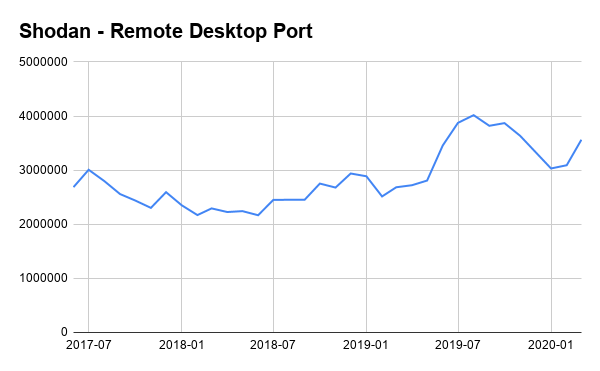
\includegraphics[width=\textwidth]{img/tables/01_Shodan-RDP.png}
         \caption{RDP expuesto.}
         \label{fig:puerto 3389 expuesto}
     \end{subfigure}
     \begin{subfigure}[b]{0.3\textwidth}
         \centering
         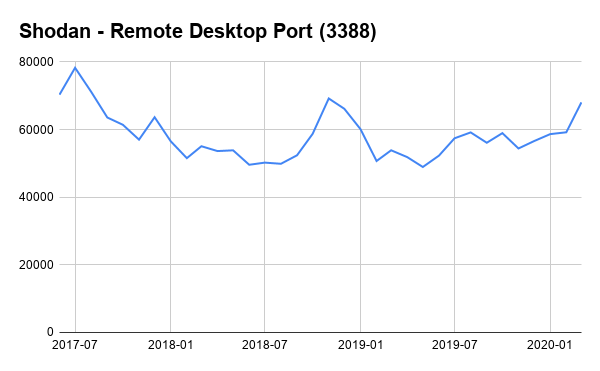
\includegraphics[width=\textwidth]{img/tables/02_Shodan-RDP-alt.png}
         \caption{RDP expuesto. (alt.)}
         \label{fig:puerto 3388 expuesto}
     \end{subfigure}
     \begin{subfigure}[b]{0.3\textwidth}
        \centering
        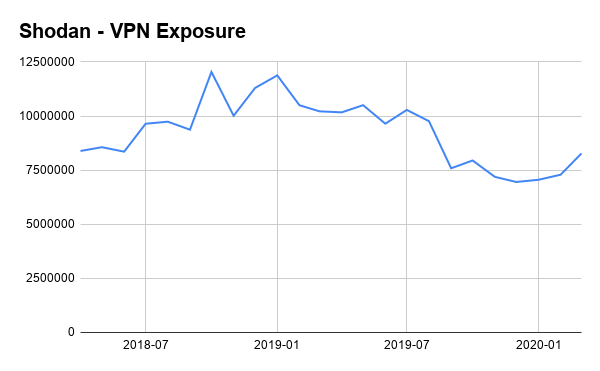
\includegraphics[width=\textwidth]{img/tables/03_Shodan-VPN.png}
        \caption{VPN expuesto.}
        \label{fig:servicio vpn expuesto}
     \end{subfigure}
    \caption{Cantidad de dispositivos según el servicio expuesto. Fuente: \textit{Shodan}.}
    \label{fig:servicios expuestos}
\end{figure}

La actual pandemia también ha tenido un gran impacto en la ciberseguridad. Los ataques informáticos contra corporaciones, así como las estafas en línea, se dispararon en más de un 400\% en marzo de 2020 en comparación con los meses anteriores, según la firma de abogados internacional \textit{Reed Smith} \cite{reedsmithcovidfraud}, mientras que \textit{Google} reveló que estaba bloqueando más de 18 millones de correos electrónicos de malware y phishing relacionados con el COVID-19 cada día \cite{googlecovidfraud}.\sn

Los ciberdelincuentes  siguen consiguiendo comprometer los datos y sistemas corporativos con relativa facilidad y de forma regular. Esto se debe a la falta de perfiles cualificados que sean capaces de realizar auditorías de seguridad (o \textit{pentestings}), con el fin de asegurar los activos de la compañía \cite{cybersecurityspecialist}. Además, las tácticas empleadas por los ciberdelincuentes son cada vez más sofisticadas, haciendo que este tipo de ejercicios se vuelvan a su vez más complejos y extensos. \textit{Gartner} ha proyectado que las empresas invirtieron más de 123.000 millones de dólares en ciberseguridad en 2020 \fig{cybersecuritybudget} y prevé que esa cifra aumente a 170.400 millones de dólares en 2022 \cite{cibersecuritybudget}.\n

\begin{figure}[h]
    \centering
    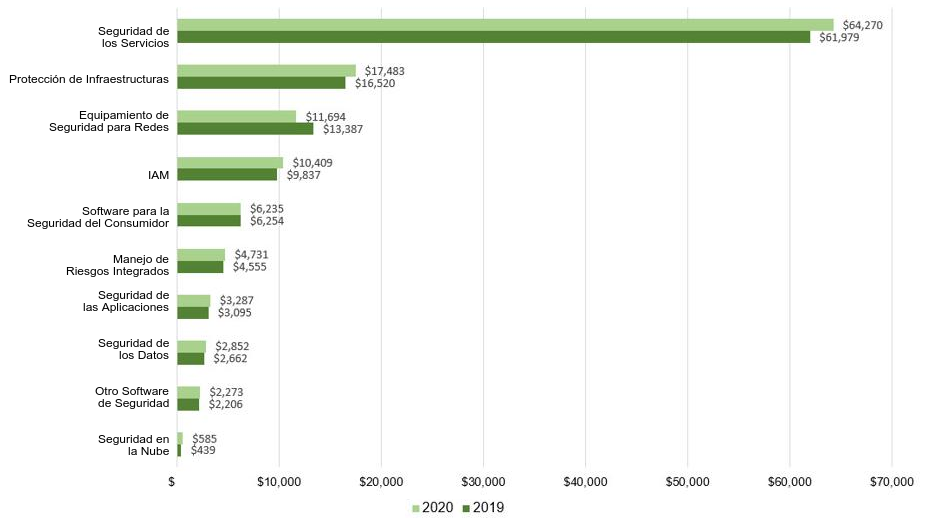
\includegraphics[width=15cm]{img/tables/04_Cybersecurity-Budget.png}
    \caption{Gasto mundial en ciberseguridad (en millones de dólares). Fuente: \textit{Forbes}.}
    \label{fig:cybersecuritybudget}
\end{figure}

%%%%%%%%%%%%%%%%%%%%%%%%%%%%%
%% Motivation
%%%%%%%%%%%%%%%%%%%%%%%%%%%%%

\section{Motivación} \label{sec:motivación}

La seguridad informática es un campo cambiante y en constante crecimiento. La complejidad a la hora de realizar ejercicios de intrusión requiere que los auditores tengan acceso a un amplio repertorio de herramientas, donde cada una de las cuales generalmente está enfocada en tareas concretas dentro de la totalidad de la auditoría.\sn

Además, el autor de este documento también ha experimentado la dificultad a la que se enfrenta un docente al intentar formar nuevos perfiles dentro del campo de la ciberseguridad.\sn

Esto se debe a que las soluciones \textit{software} actuales requieren de conocimientos informáticos avanzados, tienen una funcionalidad muy específica o sólo están disponibles para arquitecturas de sistemas concretos.



%%%%%%%%%%%%%%%%%%%%%%%%%%%%%
%% Objetives
%%%%%%%%%%%%%%%%%%%%%%%%%%%%%

\section{Objetivo} \label{sec:objetivos}

Este Trabajo de Fin de Grado se plantea con el objetivo de crear un proyecto de código abierto enfocado a la seguridad informática, que automatice y enlace varias de las etapas más habituales durante un \textit{pentesting} (listado de subdominios y servicios, comprobación de filtrados de información, credenciales por defecto, vulnerabilidades conocidas...), y que su uso sea válido tanto en auditorías reales como en entornos educativos, con el fin de simplificar y desmitificar las actividades relacionadas con el mundo de la ciberseguridad, acorde a lo detallado en el apartado \ref{sec:motivación}.\n

\subsection{Objetivos específicos} \label{sub:objetivosespecificos}

Además de llevar a cabo el proyecto, existen una serie de especificaciones que ha de cumplir el programa. Dichos requisitos, detallados a continuación, son necesarios para asegurarse de que la funcionalidad es acorde a la motivación inicial por parte del autor.\sn

\subsubsection{Manejo visual e intuitivo} \label{subsub:objvisual}

Debido a que una de las motivaciones de este proyecto es acercar el mundo de la ciberseguridad a aquellos perfiles ajenos al sector, es necesaria la opción de poder prescindir de la habitual línea de comandos. Una alternativa es reemplazarla por una interfaz gráfica, teniendo como preferencia un diseño similar a un lenguaje de programación visual. Como ejemplo de lenguajes visuales, se encuentran aquellas basadan en bloques (véase \textit{Scratch}\footnote{\url{https://scratch.mit.edu/}} o \textit{AppInventor}\footnote{\url{https://appinventor.mit.edu/}}), o basadas en nodos (\textit{Node-RED}\footnote{\url{https://nodered.org/}} o \textit{vvvv}\footnote{\url{https://vvvv.org/}}), entre otros, siendo este último la preferencia.\sn

Además, se pretende que al aproximarse a este concepto, la aplicación ofrezca una experiencia de usuario similar a la de ``crear recetas'', pudiendo compartirlas y reduciendo así el tiempo requerido para realizar auditorías de seguridad.\sn

\subsubsection{Estandarización de tareas} \label{subsub:objapi}

Se requiere que la aplicación ejecute tareas repetitivas, pertenecientes a las diferentes etapas de una auditoría de ciberseguridad, que interactúan directamente con servicios y dispositivos externos.\sn

Para ello, será necesaria la creación de una \textbf{Interfaz de Programación de Aplicaciones} (\textit{API} en adelante). Proporcionará una manera sencilla de realizar dichas tareas mediante llamadas estandarizadas a la aplicación, independientemente del servicio o dispositivo auditado.\sn

\subsubsection{Distribución sencilla} \label{subsub:objdist}

Acorde a la motivación mencionada en el apartado \ref{subsub:objvisual}, se requiere que la distribución de la aplicación sea lo más sencilla posible. Para ello, se tendrá como objetivo la compilación de todo el entorno en un único ejecutable, sin dependencias, y con soporte para los sistemas operativos y arquitecturas más populares.\sn

Este aspecto también concuerda con la ideología de crear un programa que sirva de reemplazo para gran parte de las soluciones existentes actualmente en el mercado, al poder ejecutar varias de las tareas habituales durante una auditoría de seguridad desde una misma plataforma que no dependa de programas externos.\n

%%%%%%%%%%%%%%%%%%%%%%%%%%%%%
%% Technical description
%%%%%%%%%%%%%%%%%%%%%%%%%%%%%

\section{Descripción técnica} \label{sec:desctecnica}

En este punto se especifican, de manera breve, los componentes que formarán la aplicación con el fin de contextualizar los siguientes capítulos. Los requisitos serán explicados en profundidad en los apartados \ref{sec:userrequirements} y \ref{cap:requirements}, así como la arquitectura y el diseño de la misma (apartados \ref{cap:arch} y \ref{cap:design}, respectivamente). La solución propuesta en este documento constará, según la naturaleza de sus componentes, de varios elementos.\sn

Si aplicamos una categorización basada en soluciones software con interfaz gráfica, podemos diferenciar la aplicación en dos partes: la \textbf{interfaz} (o \textit{frontend}) y el \textbf{servidor} (o \textit{backend})\footnote{Puede ser objeto de debate definir a qué categoría pertenece cada uno de los elementos que conforman la aplicación. En este documento, se atribuyen al \textit{frontend} todos aquellos elementos desarrollados mediante el uso de \textit{HTML}, \textit{CSS} y/o \textit{JavaScript}. El resto, se asocian con el \textit{backend}.}.\sn
 
Por otro lado, siguiendo una categorización enfocada en la utilidad, podemos diferenciar tres entidades \fig{mockuputility}:\sn

\begin{figure}[H]
    \centering
    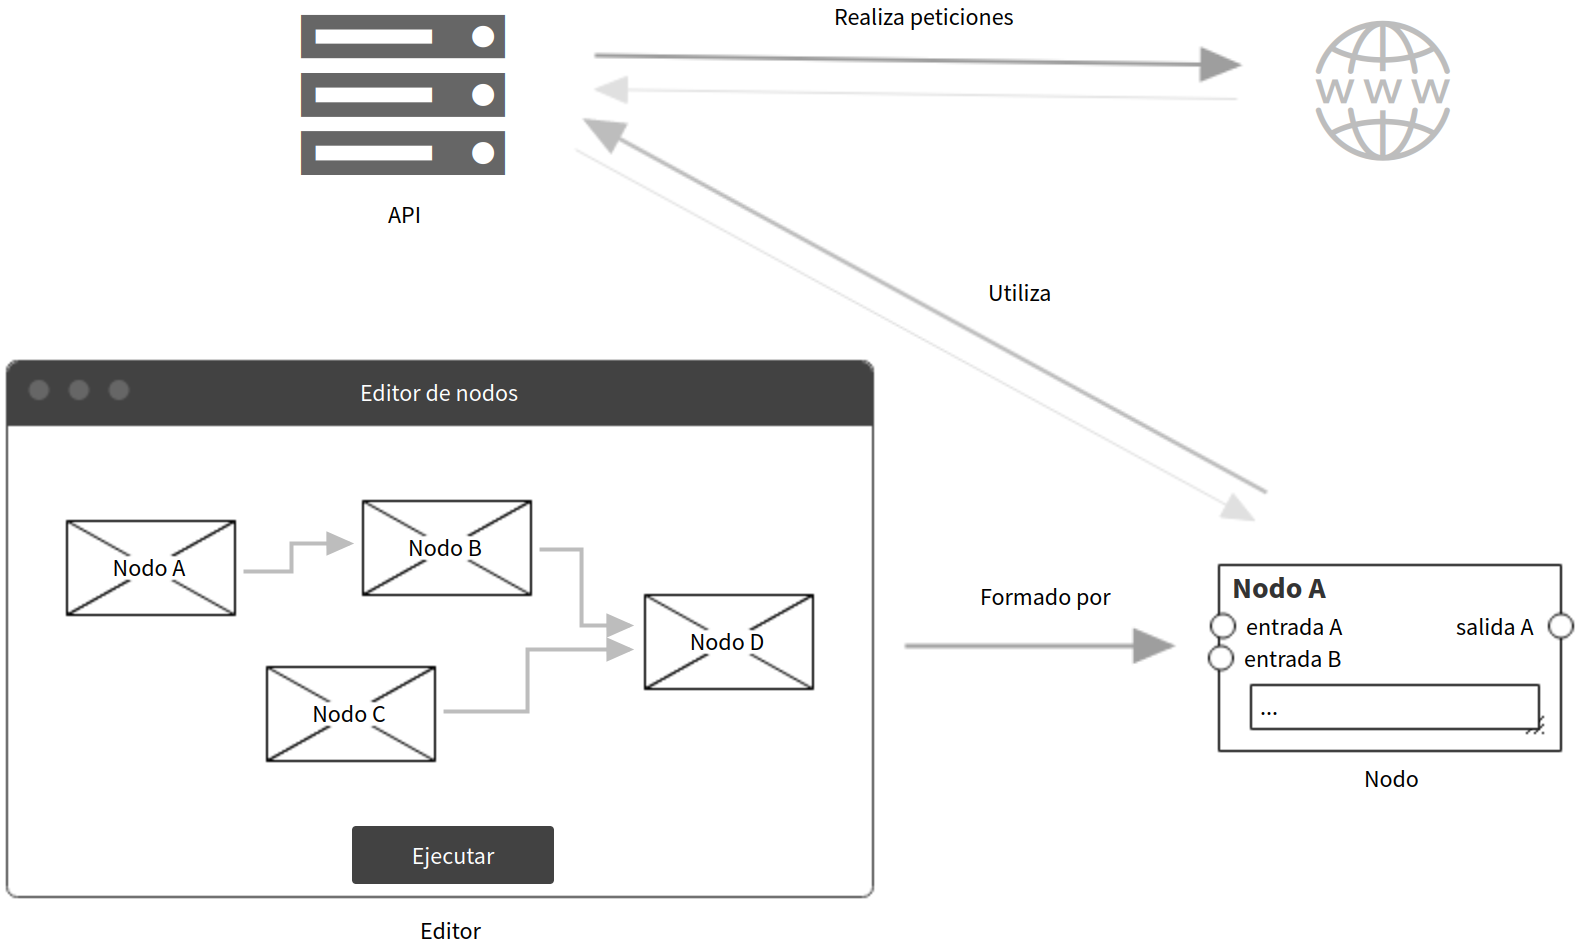
\includegraphics[width=11cm]{img/tables/05_Mockup-Utility.png}
    \caption{\textit{Mockup} según la utilidad de los componentes.}
    \label{fig:mockuputility}
\end{figure}


- La \textbf{\textit{API}}, encargada de manejar las peticiones y proporcionar los datos referentes a sistemas externos a la aplicación.\sn

- Los \textbf{nodos}, encargados de encapsular tareas concretas, de las cuales se pueden obtener datos a través de ciertos valores de entrada y/o parámetros de configuración (similar a la idea de \textit{función} dentro de la programación).\sn

- El \textbf{editor de nodos}, encargado de interpretar los nodos, interconectarlos entre si, manejar el flujo de datos y controlar la ejecución del programa.\n

Además, los componentes (así como la solución final) deberán cubrir una serie de características técnicas detalladas a continuación.

\subsection{Interfaz de Programación de Aplicaciones / API} \label{sub:api}

La \textbf{API} es, posiblemente, una de las partes más delicadas en cuanto a su diseño se refiere. Será la encargada de interactuar con los activos auditados, por lo que su implementación deberá ser precisa para evitar conexiones innecesarias y/o pérdidas en el contenido de los datos recibidos. Un mal diseño no sólo ralentizaría el servicio, sino que podría sobreexponer al auditor, además de causar daños sobre los activos.\sn

Muchas de las tareas habituales durante una auditoría de ciberseguridad no requieren de una conexión activa. Es por ello que las peticiones realizadas deberán cerrarse una vez finalizadas. En el caso de que se exija más información sobre el mismo activo se podrán reusar, siempre que sea posible, las respuestas entre las tareas que auditen características similares. De esta forma se consigue evitar la sobrecarga.\sn

La ejecución de las rutinas encargadas de realizar las conexiones se estandarizarán usando el protocolo \textit{HTTP}. Ésto se podrá conseguir mediante la creación de un servicio que tramite cada una de las peticiones y devuelva los resultados en formato \textit{JSON}.\sn

Para abarcar de manera satisfactoria estos problemas, se pretende utilizar un lenguaje de programación con acceso a librerías que permitan la creación de tramas a bajo nivel. De esta forma, se logrará obtener un mayor control sobre los datos enviados.\sn

Por otro lado, la velocidad de ejecución es un tema a tener en cuenta, dado que se realizarán múltiples tareas en un periodo de tiempo limitado. Por lo tanto, el lenguaje seleccionado debe ser compilado (dado que ofrece un mayor rendimiento frente a las alternativas interpretadas), y con soporte para modelos de computación no secuenciales (\textit{concurrencia} o \textit{paralelismo}, por ejemplo).\sn

También se pretende minimizar el riesgo de errores durante la ejecución, por lo que el lenguaje ha de ser \textit{tipado} (variables con tipos definidos) y que ofrezca mecanismos de gestión de excepciones.\sn

Ejemplos de lenguajes de programación que cumplen con estos requisitos son, entre otros: \textit{C/C++}, \textit{Rust} o \textit{Golang}.

\subsection{Editor de nodos} \label{sub:nodeeditor}

Este componente tendrá que encargarse de interpretar correctamente los nodos que lo conforman. Permite, a su vez, realizar operaciones de conexión y desconexión entre dos o más nodos, así como la personalización de los valores asociados a cada uno de ellos.\sn

El diseño seleccionado para el editor seguirá el paradigma de programación de flujo de datos (o \textit{dataflow programming}), el cual modela un programa como un gráfico dirigido en el que los datos fluyen entre las operaciones.\sn

Aunque existen varios patrones de diseño relacionados con este paradigma, se valorarán principalmente dos de ellos para la implementación: los basados en un único flujo de datos unidimensional (totalmente lineal), y los basados en nodos interconectados entre sí, formando un gráfico bidimensional con varios flujos de datos simultáneos \fig{mockupdataflow}.\sn

\begin{figure}[h]
    \centering
    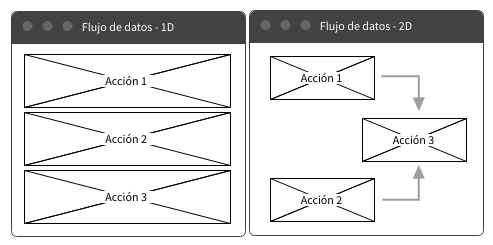
\includegraphics[width=10cm]{img/tables/06_Mockup-Dataflow-Types.png}
    \caption{\textit{Mockup} según el patrón de diseño.}
    \label{fig:mockupdataflow}
\end{figure}
\vspace{0.3cm}

Las aplicaciones con diseños unidimensionales\footnote{Un ejemplo de esta implementación es \textit{Cyberchef} (\url{https://gchq.github.io/CyberChef/})} son más intuitivas al compartir los datos en una única dirección, pero exige que todas las acciones sean evaluadas en el orden definido, existiendo un solo flujo de ejecución.\sn

Por el contrario, las soluciones con diseños bidimensionales ofrecen un mayor control sobre el orden de ejecución, pero su implementación requiere de un mayor esfuerzo, debido a que es necesario controlar excepciones tales como bucles infinitos, acciones huérfanas o flujos de datos independientes, entre otras \fig{mockupdataflowerrors}.\sn

\begin{figure}[H]
    \centering
    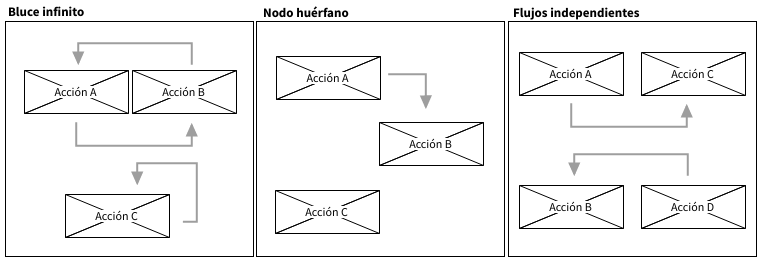
\includegraphics[width=11cm]{img/tables/07_Mockup-Dataflow-Problems.png}
    \caption{\textit{Mockup} de errores comunes al desarrollar diseños bidimensionales.}
    \label{fig:mockupdataflowerrors}
\end{figure}

Para la implementación de este diseño, es necesario que el lenguaje de programación seleccionado conste de librerías que permitan el desarrollo de interfaces altamente personalizables. Los lenguajes como \textit{Golang} o \textit{Rust}, mencionados en el apartado \ref{sub:api}, carecen de dichas librerías\footnote{Algunos de ellos ni siquiera ofrecen soporte gráfico, como \textit{Rust}. (\url{https://www.areweguiyet.com/})}, por lo que también se valorará realizar la interfaz mediante lenguajes web.\sn

Los nodos deberán seguir un estándar y ofrecer la capacidad de definir nuevos a través del uso de archivos parametrizados que consten, por ejemplo, de los siguientes valores:\sn

- \textbf{Identificador}: Cadena única usada para referenciar al nodo.

- \textbf{Nombre}: Texto identificativo mostrado en el editor.

- \textbf{Categoría}: Grupo al que pertenece según su funcionalidad.

- \textbf{Descripción}: Documentación relativa a su utilidad.

- \textbf{Etiquetas}: Palabras descriptivas por las que filtrar al nodo.

- \textbf{Entradas}: Valores de entrada requeridos.

- \textbf{Salidas}: Valores resultantes de la ejecución del nodo.

- \textbf{Controles}: Parámetros de configuración.

- \textbf{Código}: Método utilizado para generar los valores de salida.\sn

Los flujos de datos también deberán poder exportarse e importarse mediante ficheros, los cuales especificarán, al menos:\sn

- \textbf{Identificador}: Cadena usada para referenciar los tipos de nodos soportados.

- \textbf{Nodos}: Resumen de los nodos presentes en el editor, así como las conexiones entre ellos.\n

\subsection{Binario precompilado multiplataforma} \label{sub:binary}

De acuerdo al objetivo detallado en el punto \ref{subsub:objdist}, la aplicación ha de ser fácil de distribuir. Para ello, será necesario que el lenguaje seleccionado sea capaz de procesar plantillas \textit{HTML}. Dichas plantillas formarán parte del código fuente, con la intención de reducir el número de archivos que formen la aplicación a un único fichero ejecutable. Además, esto requiere que sea un lenguaje compilado, al igual que en el apartado \ref{sub:api}.\sn

Por otro lado, el programa ha de ser multiplataforma y sin dependencias de librerías o programas externos.\sn

Existen compiladores (como el nativo de \textit{Golang}) que permiten generar binarios teniendo como objetivo cualquier sistema operativo y plataforma, independientemente de la arquitectura del sistema anfitrión.\n

%%%%%%%%%%%%%%%%%%%%%%%%%%%%%
%% Laws
%%%%%%%%%%%%%%%%%%%%%%%%%%%%%

\section{Aspectos legales} \label{sec:legal}

A continuación se detallan los aspectos legales asociados al proyecto. Debido a la naturaleza del mismo, \textbf{el uso de la aplicación resultante puede ser un acto constitutivo de delito}, según la regulación de cada país.\sn

En España, se entiende por \textbf{Delito Informático} todo aquel ataque que se produce contra el derecho a la intimidad, delitos de descubrimiento y revelación de secretos mediante el apoderamiento y difusión de datos reservados registrados en ficheros o soportes informáticos. (\textit{Art.197-201 Código Penal} \cite{LO1995}).\sn

Concretamente, considera delito de \textbf{sabotaje informático} a toda aquella acción que produzca daños mediante la destrucción o alteración de datos, programas o documentos electrónicos contenidos en redes o sistemas informáticos (\textit{Art. 263} \cite{LO1995}), y delito de \textbf{fraude informático} a las estafas a través de la manipulación de datos o programas para la obtención de un lucro ilícito (\textit{Art. 248}\cite{LO1995}).\sn

Además, en la reforma realizada en 2010 \cite{LO2010}, la detección de vulnerabilidades informáticas se considera acto de delito. Cualquier persona que detecte vulnerabilidades en aplicaciones o sitios web, sin consentimiento explícito de los interesados, puede acabar con consecuencias legales. En otras palabras, \textbf{realizar un acceso no consentido, sin autorización, será considerado hecho válido de sanción, aunque no exista intención de cometer un delito}. El usuarios que comete el acto puede ser sancionado con una pena de prisión de entre seis meses y dos años.\sn

Las personas jurídicas dedicadas a la seguridad informática deben conocer esta ley, y todas las consecuencias que pueden ocurrir en el incumplimiento de la misma. Es recomendable que cualquier individuo al cargo de una auditoría de seguridad sea informado y tenga consciencia de ello, entendiendo el ámbito en el que se encuentra y a las leyes que está sujeto. Actualmente, el Código Penal no hace distinción entre un investigador de seguridad que actúa sin consentimiento y un delincuente que se aprovecha de las vulnerabilidades para obtener beneficio propio.\sn

Respecto al uso de la aplicación producto del proyecto, \textbf{el autor de este documento no se hace responsable en caso de que se presenten cargos penales contra cualquier individuo o corporación que utilice la herramienta en contra de las leyes estipuladas}, así como de los daños causado por un mal uso de la misma. Es responsabilidad del usuario final obedecer todas las leyes aplicables.\sn

Se recomienda que su uso sea limitado a entornos controlados, tales como entornos educativos, y/o pruebas de intrusión bajo autorización previa de los interesados.\n

%%%%%%%%%%%%%%%%%%%%%%%%%%%%%
%% Structure
%%%%%%%%%%%%%%%%%%%%%%%%%%%%%

\section{Organización de la documentación} \label{sec:structure}

A continuación se detalla la documentación relativa al proyecto, así como su estructura.\sn

\subsection{Memoria del proyecto} \label{sub:memo}

Se trata del documento actual. En él se recogen formalmente todos los aspectos del proyecto, desde sus primeras fases, así como las decisiones arquitectónicas tomadas, el proceso completo de desarrollo, la documentación generada y las conclusiones a
las que se han llegado como consecuencia de la realización del ejercicio.\sn

Además, se adjuntan tres anexos correspondientes a:\sn

- \textbf{Anexo A}: La bibliografía consultada durante la investigación inicial.\sn

- \textbf{Anexo B}: El manual de usuario para la correcta instalación y uso del producto desarrollado.\sn

- \textbf{Anexo C}: Resumen de los controles típicos durante una auditoría de seguridad web según la metodología descrita en la \textit{OWASP Web Security Testing Guide}\cite{owaspwstg}.\n

\subsection{Documentación del código} \label{sub:codecomments}

El código de la aplicación se ha comentado detallando las funcionalidades de las partes más importantes.\sn

Es posible visualizar de forma \textit{online} a la documentación de las clases definidas en el apartado \ref{fig:classdiagramserver}. La \textit{URL} de acceso es: \url{https://pkg.go.dev/github.com/cosasdepuma/masterchef}.\sn

Por otro lado, se pone a disposición del usuario el archivo \textit{swagger.yml}. Esto permite documentar las llamadas a la \textit{API}, usando la tecnología descrita en el apartado \ref{sec:swagger}.\n

\subsection{Repositorio público} \label{sub:repo}

Debido a que éste es un proyecto de código abierto, todos los archivos a los que se hacen referencia en esta memoria se encuentran alojados en un repositorio público. Se puede consultar y realizar un seguimiento, a través de: \url{https://github.com/CosasDePuma/Masterchef}.
    \blankpage
    %%%%%%%%%%%%%%%%%%%%%%%%%%%%%%%%%%%%%%%%%%%%%%%%%%%%%%%%%%%%%%%%%%
%%  ~ Trabajo de Fin de Grado - Universidad de Vigo (ESEI) ~    %%
%% Autor: Diego Enrique Fontán Lorenzo                          %%
%% Tutor: Miguel Ramón Díaz-Cacho Medina                        %%
%% Convocatoria: Julio 2020/21                                  %%
%% Título: Framework de automatización de auditorías Red Team   %%
%%%%%%%%%%%%%%%%%%%%%%%%%%%%%%%%%%%%%%%%%%%%%%%%%%%%%%%%%%%%%%%%%%

%%%%%%%%%%%%%%%%%%%%%%%%%%%%%
%% Planification
%%%%%%%%%%%%%%%%%%%%%%%%%%%%%

\chapter{Planificación y seguimiento} \label{cap:planification}

En este capítulo se detalla el la metodología de trabajo seguida para la correcta realización del mismo, así como la planificación inicial, la descripción de las fases, la recogida de requisitos y las desviaciones respecto al plan sufridas durante el proceso de desarrollo.\n

%%%%%%%%%%%%%%%%%%%%%%%%%%%%%
%% Methodology
%%%%%%%%%%%%%%%%%%%%%%%%%%%%%

\section{Metodología de trabajo} \label{sec:methodology}

A continuación se explican las metodologías utilizadas a lo largo de la vida del desarrollo de este proyecto.\sn

Dichas metodologías han sido escogidas acorde a una serie de características derivadas de la naturaleza de la aplicación desarrollada, así como las habilidades y recursos disponibles por parte del autor de este documento.\n

\subsection{Metodología \textit{eXtreme Programming}} \label{sub:methoXP}

Para el desarrollo del proyecto se ha optado por implementar la metodología de Programación Extrema (o \textit{eXtreme Programming}).\sn

Catalogada como una metodología ágil, tiene como base la simplicidad y adaptabilidad, en vez de la previsibilidad. Esto permite que sea más natural hacer cambios sobre la marcha en los requisitos, en vez de tratar de definirlos todos al comienzo del proyecto. Es decir, conforme avance el proyecto, se adaptará el código a las necesidades que vayan surgiendo.\sn

\subsubsection{Características} \label{subsub:methoXPcaract}

Sus principales características son las siguientes:\sn

- Se diseña y construye una base sólida sobre la que añadir nuevas características, mediante un \textbf{desarrollo iterativo e incremental}.\sn

- Las capturas de requisitos deben ser escritas de manera breve y usando lenguaje natural por el cliente. A cada una de estas capturas se le conoce con el nombre de \textbf{historias de usuario}. Normalmente generan una nueva funcionalidad del sistema y deben ser independientes entre sí.\n

- Apuesta por mantener el \textbf{código lo más simplificado posible}, realizando una refractorización del mismo siempre que el desarrollador lo considere adecuado.\sn

- Antes de desarrollar cualquier funcionalidad nueva, se debe establecer un conjunto de objetivos, así como una \textbf{batería de pruebas unitarias}, preferiblemente automatizadas.\sn

- Antes de generar una nueva característica, es necesario \textbf{corregir todos los errores detectados en la iteración actual}, además de revisar y documentar cada una de las pruebas unitarias.\sn

- Se prioriza generar la \textbf{documentación de manera} integrada en los archivos fuente del \textit{software} y de forma simultánea al desarrollo, de manera que no existan iteraciones con segmentos de código sin documentar.\sn

- La \textbf{integración del cliente como parte del equipo} es necesaria para saber si el requerimiento cumple con las expectativas.\sn

- Se recomienda la \textbf{programación en parejas}, donde ambos integrantes comparten las actividades y responsabilidades referentes a un mismo código o proyecto.\n

\subsubsection{Limitaciones} \label{subsub:methoXPlimit}

Si bien la metodología expuesta encaja con el proyecto propuesto, no todas las características descritas en el apartado \ref{subsub:methoXPcaract} se ajustan a las restricciones inherentes a un Trabajo de Fin de Grado.\sn

En este caso concreto, el desarrollo de la aplicación no sigue la recomendación de la programación en parejas. Todo el proceso ha sido llevado a cabo por una única persona (el autor de este documento).\sn

Por otro lado, debido a que el cliente interesado en el producto no puede definirse con exactitud\footnote{Dependiendo de la opinión personal de cada lector, el cliente podría considerarse la propia Universidad, el tutor del proyecto o el público objetivo del trabajo, entre otros.}, se ha designado que sea el tutor del proyecto quien se encargue este rol, teniendo en cuenta las limitaciones de horarios y medios del mismo. El resto de roles pertenecientes a un equipo basado en esta metodología (\textit{Tester}, \textit{Coach}, \textit{Manager}...) recaen bajo el autor del trabajo.\sn

Por último, también será el autor quien genere gran parte de las historias de usuario, dado que se trata de un proyecto propio, el cual no ha sido propuesto por el tutor ni la Universidad.

\subsection{Anexo: Metodología \textit{SCRUM}} \label{sub:methoSCRUM}

Debido a que la documentación generada usando la metodología propuesta en el apartado \ref{sub:methoXP} no contempla de manera detallada la planificación del trabajo mediante la distribución en fases y tareas propias de un Trabajo de Fin de Grado, se ha optado por complementar este paradigma con otro proceso alternativo: la metodología \textit{SCRUM}.\sn

\subsubsection{Características} \label{subsub:methoSCRUMcaract}

Las características implementadas en este proyecto son:\sn

- El desarrollo incremental de los requisitos del proyecto se organiza en \textbf{bloques temporales cortos y fijos}.\sn

- Se establecen \textbf{tiempos máximos para lograr objetivos}.\sn

- \textbf{Se agrupan las tareas independientes en \textit{sprints}}, que a su vez harán de iteraciones.\sn

Dichas características son aplicadas solamente para la documentación del proyecto, dado que el desarrollo se llevará a cabo respecto a lo mencionado en el apartado \ref{sub:methoXP}.\n

%%%%%%%%%%%%%%%%%%%%%%%%%%%%%
%% Initial plan
%%%%%%%%%%%%%%%%%%%%%%%%%%%%%

\section{Planificación inicial} \label{sec:initialplan}

El desarrollo de la aplicación se ha dividido en ocho partes, con una estimación temporal asociada a cada una de ellas en función de la carga de trabajo \tab{initialplan}, con jornadas de ocho horas y semanas laborables de cinco días.\sn

\begin{table}[ht]
    \begin{center}
        \begin{tabular}{| l | c |}
            \hline
            \textbf{Iteración} & \textbf{Estimación} (en horas) \\
            \hline
            Investigación inicial                   & 32.0   \\ \hline
            Especificación de requisitos            & 16.0   \\ \hline
            Diseño del \textit{software}            & 24.0   \\ \hline
            \textit{Sprint} 1: Implementación de la interfaz & 80.0  \\ \hline
            \textit{Sprint} 2: Implementación de la \textit{API}      & 48.0   \\ \hline
            \textit{Sprint} 3: Implementación de los nodos   & 40.0   \\ \hline
            \textit{Sprint} 4: Integración del sistema       & 24.0   \\ \hline
            Elaboración del documento               & 96.0  \\ \hline
            \textbf{Total}                          & 360.0 \\ \hline
        \end{tabular}
    \end{center}
    \caption{Estimación temporal según la planificación inicial.}
    \label{tab:initialplan}
\end{table}
\vspace{1cm}

\subsection{Diagrama de Gantt} \label{sub:gantt}

A continuación se muestra la planificación temporal mediante un cronograma \fig{gantt}. El eje horizontal está asociado con el marco del tiempo (en días) y, el vertical, con cada una de las iteraciones.\sn

\begin{figure}[h]
    \centering
    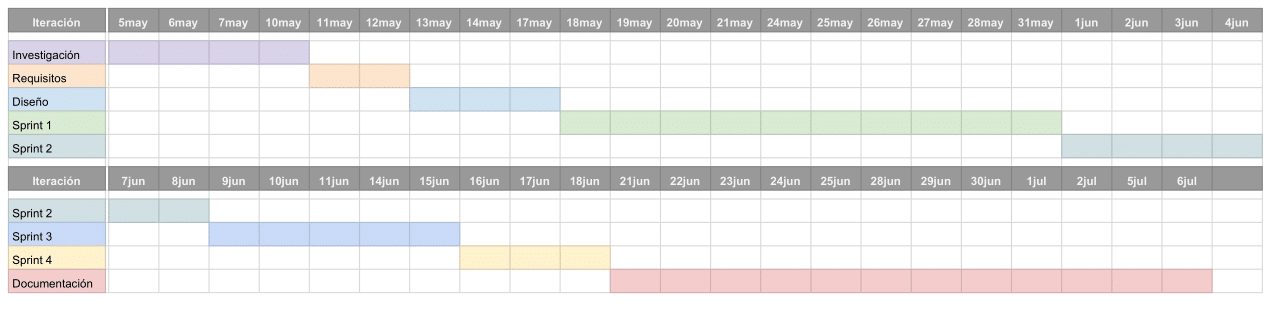
\includegraphics[width=15cm]{img/tables/08_Planned-Gantt.png}
    \caption{Diagrama de Gantt.}
    \label{fig:gantt}
\end{figure}

%%%%%%%%%%%%%%%%%%%%%%%%%%%%%
%% Phases
%%%%%%%%%%%%%%%%%%%%%%%%%%%%%

\section{Descripción de las fases} \label{sec:phases}

En este punto se procede a detallar cada una de las iteraciones descritas en el apartado \ref{sec:initialplan}. Además, por cada iteración, se definirán una serie de subtareas junto a su estimación temporal.\n

\subsection{Investigación inicial} \label{sub:initialinv}

Primera fase del proceso de desarrollo mediante la cual se realizará el estudio del arte, tomando como antecedentes aquellos proyectos que compartan características similares a la idea propuesta, ya sea en su motivación o en su implementación. Durante esta fase también se valorarán todos los conceptos relativos a lenguajes de programación, protocolos, patrones de diseño y metodologías que puedan ser objeto de interés durante el desarrollo.\sn

Las tareas asociadas a esta fase son:\sn

\begin{table}[ht]
    \begin{center}
        \begin{tabular}{| l | c |}
            \hline
            \textbf{Tarea} & \textbf{Estimación} (en horas) \\
            \hline
            Investigación sobre \textit{software} similar & 8.0 \\ \hline
            Investigación técnica   & 12.0 \\ \hline
            Investigación legal     & 4.0 \\ \hline
            Documentación relativa a ciberseguridad & 8.0 \\ \hline
            \textbf{Total}          & 32.0 \\ \hline
        \end{tabular}
    \end{center}
    \caption{Tareas y estimación temporal de la investigación inicial.}
    \label{tab:phase1}
\end{table}

\subsection{Especificación de requisitos} \label{sub:requirements}

La fase de especificación de requisitos consiste en la creación de las historias de usuario iniciales, las cuales formarán el núcleo de la aplicación. También se encargará de definir las herramientas necesarias para la realización del trabajo.\sn

Las tareas asociadas a esta fase son:\sn

\begin{table}[ht]
    \begin{center}
        \begin{tabular}{| l | c |}
            \hline
            \textbf{Tarea} & \textbf{Estimación} (en horas) \\
            \hline
            Definición de las historias de usuario  & 8.0 \\ \hline
            Definición de tecnologías y lenguajes   & 4.0 \\ \hline
            Planificación de los \textit{sprints}   & 4.0 \\ \hline
            \textbf{Total}                          & 16.0 \\ \hline
        \end{tabular}
    \end{center}
    \caption{Tareas y estimación temporal de la especificación de requisitos.}
    \label{tab:phase2}
\end{table}

\subsection{Diseño de la aplicación} \label{sub:appdesign}

En esta fase se valorará la arquitectura inicial de la aplicación. Es necesaria para concretar las bases sobre las que se comenzará a desarrollar el programa. Aún así, al tratarse de la metodología \textit{eXtreme Programming}, es posible que ésta se transforme a lo largo de todo el proceso de desarrollo.\sn

Las tareas asociadas a esta fase son:\sn

\begin{table}[ht]
    \begin{center}
        \begin{tabular}{| l | c |}
            \hline
            \textbf{Tarea} & \textbf{Estimación} (en horas) \\
            \hline
            Diseño de la arquitectura               & 12.0 \\ \hline
            Bocetaje de posibles flujos de datos    & 8.0 \\ \hline
            Bocetaje de la interfaz                 & 4.0 \\ \hline
            \textbf{Total}                          & 24.0 \\ \hline
        \end{tabular}
    \end{center}
    \caption{Tareas y estimación temporal del diseño de la aplicación.}
    \label{tab:phase3}
\end{table}

\subsection{\textit{Sprint} 1 - Implementación de la interfaz} \label{sub:sprint1}

El primer \textit{sprint} está dedicado a la creación de la interfaz visual. Se encargará de implementar cómo interpretará la aplicación el flujo de datos y todo lo referente a la interacción con el usuario.\sn

A pesar de tratarse de una aplicación híbrida, y al contrario que en los procesos de desarrollo de aplicaciones para escritorio (donde la interfaz generalmente es lo último en implementarse), se ha optado por una aproximación similar al proceso de desarrollo web, en el que el \textit{frontend} es el protagonista.\n

Las tareas asociadas a esta fase son:\sn

\begin{table}[ht]
    \begin{center}
        \begin{tabular}{| l | c |}
            \hline
            \textbf{Tarea} & \textbf{Estimación} (en horas) \\
            \hline
            Creación de pruebas unitarias       & 8.0 \\ \hline
            Diseño del modelo de flujo de datos & 36.0 \\ \hline
            Implementación del flujo de datos   & 16.0 \\ \hline
            Diseño de la interfaz gráfica       & 20.0 \\ \hline
            \textbf{Total}                      & 80.0 \\ \hline
        \end{tabular}
    \end{center}
    \caption{Tareas y estimación temporal de la implementación de la interfaz.}
    \label{tab:phase4}
\end{table}

\subsection{\textit{Sprint} 2 - Implementación de la \textit{API}} \label{sub:sprint2}

El segundo \textit{sprint} está dedicado a la creación de la \textit{API}. Se encargará de crear el servidor \textit{HTTP}, definir el enrutamiento e implementar las peticiones a terceros.\sn

Las tareas asociadas a esta fase son:\sn

\begin{table}[ht]
    \begin{center}
        \begin{tabular}{| l | c |}
            \hline
            \textbf{Tarea} & \textbf{Estimación} (en horas) \\
            \hline
            Creación de pruebas unitarias       & 8.0 \\ \hline
            Implementación del servidor         & 12.0 \\ \hline
            Implementación del \textit{router}  & 12.0 \\ \hline
            Implementación de los \textit{middlewares} & 4.0 \\ \hline
            Implementación de las acciones relativas a terceros & 12.0 \\ \hline
            \textbf{Total}                          & 48.0 \\ \hline
        \end{tabular}
    \end{center}
    \caption{Tareas y estimación temporal de la implementación de la \textit{API}.}
    \label{tab:phase5}
\end{table}

\subsection{\textit{Sprint} 3 - Implementación de los nodos} \label{sub:sprint3}

El tercer \textit{sprint} consta de la definición de un estándar asociado a la creación de los nodos, así como la propia creación de varios nodos de ejemplo.\sn

Los tipos de nodos resultantes fruto de esta iteración formarán parte del cuerpo de la aplicación, pero se dedicará más tiempo y recursos a una sólida estandarización, con el objetivo de proporcionar a la comunidad la habilidad de diseñar, crear y compartir sus propios nodos.\sn

Las tareas asociadas a esta fase son:\sn

\begin{table}[ht]
    \begin{center}
        \begin{tabular}{| l | c |}
            \hline
            \textbf{Tarea} & \textbf{Estimación} (en horas) \\
            \hline
            Creación de pruebas unitarias       & 8.0 \\ \hline
            Estandarización de los nodos        & 16.0 \\ \hline
            Implementación de los nodos         & 8.0 \\ \hline
            Creación de varios nodos de ejemplo & 8.0 \\ \hline
            \textbf{Total}                      & 40.0 \\ \hline
        \end{tabular}
    \end{center}
    \caption{Tareas y estimación temporal de la implementación de los nodos.}
    \label{tab:phase6}
\end{table}

\subsection{\textit{Sprint} 4 - Integración del sistema} \label{sub:sprint4}

El último \textit{sprint} corresponde a la interconexión de los módulos desarrollados en las etapas anteriores del desarrollo. Será el encargado de unificar la interfaz gráfica con el servidor, además de preparar los archivos necesarios para su correcta distribución.\sn

Las tareas asociadas a esta fase son:\sn

\begin{table}[ht]
    \begin{center}
        \begin{tabular}{| l | c |}
            \hline
            \textbf{Tarea} & \textbf{Estimación} (en horas) \\
            \hline
            Creación de pruebas unitarias       & 8.0 \\ \hline
            Interconexión de los módulos        & 12.0 \\ \hline
            Creación de los archivos y \textit{scripts} de distribución         & 4.0 \\ \hline
            \textbf{Total}                      & 24.0 \\ \hline
        \end{tabular}
    \end{center}
    \caption{Tareas y estimación temporal de la integración del sistema.}
    \label{tab:phase7}
\end{table}

\subsection{Elaboración de la documentación} \label{sub:makedoc}

Tras el desarrollo del proyecto, el último marco temporal está reservado para la maquetación del documento actual, así como de los Anexos y demás archivos referentes a la documentación del Trabajo de Fin de Grado.\sn

Las tareas asociadas a esta fase son:\sn

\begin{table}[ht]
    \begin{center}
        \begin{tabular}{| l | c |}
            \hline
            \textbf{Tarea} & \textbf{Estimación} (en horas) \\
            \hline
            Memoria del proyecto    & 80.0 \\ \hline
            Anexos                  & 16.0 \\ \hline
            \textbf{Total}          & 96.0 \\ \hline
        \end{tabular}
    \end{center}
    \caption{Tareas y estimación temporal de la elaboración del documento.}
    \label{tab:phase8}
\end{table}

%%%%%%%%%%%%%%%%%%%%%%%%%%%%%
%% Requirements
%%%%%%%%%%%%%%%%%%%%%%%%%%%%%

\section{Historias de usuario} \label{sec:userrequirements}

Durante la tarea descrita en el apartado \ref{sub:requirements} y en relación a la metodología usada en este proyecto (ver apartado \ref{sec:methodology}), los requisitos de la aplicación se han definido usando \textbf{historias de usuario}, que actuarán a su vez de \textit{Product  Backlog}\footnote{Listado  de todas  las  tareas  que  se  pretenden  hacer  durante  el desarrollo del proyecto.} (relativo a la metodología \textit{SCRUM}). A continuación, se detallan cada una de ellas de manera numerada siguiendo el formato \textbf{HUXX}, donde \textit{XX} corresponde a un número de identificación arbitrario\footnote{El orden de las historias de usuario no viene determinado por su orden de implementación. Para reflejar este aspecto, se ha optado por asociar cada una de ellas a los \textit{sprints} definidos en el apartado \ref{tab:initialplan}.}.\sn

Todas las historias de usuario deben comenzar por el texto ``Deseo \ldots'' y tienen una prioridad asociada del 1 al 100 (siendo 1 la más baja y 100 la más alta).\sn

Los requisitos iniciales especificados son:\sn

\begin{table}[H]
    \begin{center}
        \begin{tabularx}{\textwidth}{| l | X |}
            \hline
            \textbf{ID}             & HU01 \\ \hline
            \textbf{Título}         & Deseo que la aplicación tenga interfaz gráfica \\ \hline
            \textbf{Descripción}    & La aplicación debe poder ser manejable mediante el uso del ratón \\ \hline
            \textbf{Prioridad}      & 90 \\ \hline
            \textbf{Iteración}      & \textit{Sprint} 1 \\ \hline
        \end{tabularx}
    \end{center}
    \caption{Historia de usuario -- 01.}
    \label{tab:hu01}
\end{table}

\begin{table}[H]
    \begin{center}
        \begin{tabularx}{\textwidth}{| l | X |}
            \hline
            \textbf{ID}             & HU02 \\ \hline
            \textbf{Título}         & Deseo que sea capaz de ejecutar tareas propias de un \textit{pentesting} \\ \hline
            \textbf{Descripción}    & La aplicación debe poder realizar controles asociados a una auditoría \\ \hline
            \textbf{Prioridad}      & 99 \\ \hline
            \textbf{Iteración}      & \textit{Sprint} 2\\ \hline
        \end{tabularx}
    \end{center}
    \caption{Historia de usuario -- 02.}
    \label{tab:hu02}
\end{table}

\begin{table}[H]
    \begin{center}
        \begin{tabularx}{\textwidth}{| l | X |}
            \hline
            \textbf{ID}             & HU03 \\ \hline
            \textbf{Título}         & Deseo que se puedan declarar varios activos a auditar \\ \hline
            \textbf{Descripción}    & La aplicación debe asociar tareas a uno o más objetivos concretos \\ \hline
            \textbf{Prioridad}      & 25 \\ \hline
            \textbf{Iteración}      & \textit{Sprint} 2\\ \hline
        \end{tabularx}
    \end{center}
    \caption{Historia de usuario -- 03.}
    \label{tab:hu03}
\end{table}

\begin{table}[H]
    \begin{center}
        \begin{tabularx}{\textwidth}{| l | X |}
            \hline
            \textbf{ID}             & HU04 \\ \hline
            \textbf{Título}         & Deseo tener una lista de controles de seguridad por defecto \\ \hline
            \textbf{Descripción}    & La aplicación debe proporcionar un catálogo de tareas habituales \\ \hline
            \textbf{Prioridad}      & 60 \\ \hline
            \textbf{Iteración}      & \textit{Sprint} 3\\ \hline
        \end{tabularx}
    \end{center}
    \caption{Historia de usuario -- 04.}
    \label{tab:hu04}
\end{table}

\begin{table}[H]
    \begin{center}
        \begin{tabularx}{\textwidth}{| l | X |}
            \hline
            \textbf{ID}             & HU05 \\ \hline
            \textbf{Título}         & Deseo poder crear mis propios controles de seguridad \\ \hline
            \textbf{Descripción}    & La aplicación debe poder interpretar tareas definidas bajo un estándar \\ \hline
            \textbf{Prioridad}      & 40 \\ \hline
            \textbf{Iteración}      & \textit{Sprint} 3 \\ \hline
        \end{tabularx}
    \end{center}
    \caption{Historia de usuario -- 05.}
    \label{tab:hu05}
\end{table}

\begin{table}[H]
    \begin{center}
        \begin{tabularx}{\textwidth}{| l | X |}
            \hline
            \textbf{ID}             & HU06 \\ \hline
            \textbf{Título}         & Deseo poder ejecutar controles de manera condicional \\ \hline
            \textbf{Descripción}    & Las tareas deben poder compartir datos entre sí \\ \hline
            \textbf{Prioridad}      & 70 \\ \hline
            \textbf{Iteración}      & \textit{Sprint} 1\\ \hline
        \end{tabularx}
    \end{center}
    \caption{Historia de usuario -- 06.}
    \label{tab:hu06}
\end{table}

\begin{table}[H]
    \begin{center}
        \begin{tabularx}{\textwidth}{| l | X |}
            \hline
            \textbf{ID}             & HU07 \\ \hline
            \textbf{Título}         & Deseo poder definir el momento en el que se ejecutan las tareas \\ \hline
            \textbf{Descripción}    & La aplicación debe soportar señales de evento \\ \hline
            \textbf{Prioridad}      & 65 \\ \hline
            \textbf{Iteración}      & \textit{Sprint} 1\\ \hline
        \end{tabularx}
    \end{center}
    \caption{Historia de usuario -- 07.}
    \label{tab:hu07}
\end{table}


\begin{table}[H]
    \begin{center}
        \begin{tabularx}{\textwidth}{| l | X |}
            \hline
            \textbf{ID}             & HU08 \\ \hline
            \textbf{Título}         & Deseo poder configurar controles en base a parámetros \\ \hline
            \textbf{Descripción}    & Las tareas similares deben fusionarse en una única tarea personalizable \\ \hline
            \textbf{Prioridad}      & 10 \\ \hline
            \textbf{Iteración}      & \textit{Sprint} 3\\ \hline
        \end{tabularx}
    \end{center}
    \caption{Historia de usuario -- 08.}
    \label{tab:hu08}
\end{table}


\begin{table}[H]
    \begin{center}
        \begin{tabularx}{\textwidth}{| l | X |}
            \hline
            \textbf{ID}             & HU09 \\ \hline
            \textbf{Título}         & Deseo poder guardar plantillas de auditorías \\ \hline
            \textbf{Descripción}    & La aplicación debe proporcionar un sistema de guardado \\ \hline
            \textbf{Prioridad}      & 8 \\ \hline
            \textbf{Iteración}      & \textit{Sprint} 1\\ \hline
        \end{tabularx}
    \end{center}
    \caption{Historia de usuario -- 09.}
    \label{tab:hu09}
\end{table}

\begin{table}[H]
    \begin{center}
        \begin{tabularx}{\textwidth}{| l | X |}
            \hline
            \textbf{ID}             & HU10 \\ \hline
            \textbf{Título}         & Deseo poder compartir plantillas de auditorías \\ \hline
            \textbf{Descripción}    & La carga de plantillas debe estar sujeta a un control de versiones \\ \hline
            \textbf{Prioridad}      & 5 \\ \hline
            \textbf{Iteración}      & \textit{Sprint} 1\\ \hline
        \end{tabularx}
    \end{center}
    \caption{Historia de usuario -- 10.}
    \label{tab:hu10}
\end{table}

\begin{table}[H]
    \begin{center}
        \begin{tabularx}{\textwidth}{| l | X |}
            \hline
            \textbf{ID}             & HU11 \\ \hline
            \textbf{Título}         & Deseo que el programa no tenga dependencias \\ \hline
            \textbf{Descripción}    & La ejecución no debe depender de archivos o programas de terceros \\ \hline
            \textbf{Prioridad}      & 85 \\ \hline
            \textbf{Iteración}      & \textit{Sprint} 4\\ \hline
        \end{tabularx}
    \end{center}
    \caption{Historia de usuario -- 11.}
    \label{tab:hu11}
\end{table}

\begin{table}[H]
    \begin{center}
        \begin{tabularx}{\textwidth}{| l | X |}
            \hline
            \textbf{ID}             & HU12 \\ \hline
            \textbf{Título}         & Deseo que el programa sea multiplataforma \\ \hline
            \textbf{Descripción}    & El binario debe soportar sistemas operativos y arquitecturas populares\\ \hline
            \textbf{Prioridad}      & 80 \\ \hline
            \textbf{Iteración}      & \textit{Sprint} 4\\ \hline
        \end{tabularx}
    \end{center}
    \caption{Historia de usuario -- 12.}
    \label{tab:hu12}
\end{table}

\begin{table}[H]
    \begin{center}
        \begin{tabularx}{\textwidth}{| l | X |}
            \hline
            \textbf{ID}             & HU13 \\ \hline
            \textbf{Título}         & Deseo poder auditar objetivos que no pertenezcan a mi red local \\ \hline
            \textbf{Descripción}    & La aplicación debe poder realizar peticiones a través de Internet \\ \hline
            \textbf{Prioridad}      & 95 \\ \hline
            \textbf{Iteración}      & \textit{Sprint} 2\\ \hline
        \end{tabularx}
    \end{center}
    \caption{Historia de usuario -- 13.}
    \label{tab:hu13}
\end{table}

\begin{table}[H]
    \begin{center}
        \begin{tabularx}{\textwidth}{| l | X |}
            \hline
            \textbf{ID}             & HU14 \\ \hline
            \textbf{Título}         & Deseo poder recopilar información de fuentes abiertas \\ \hline
            \textbf{Descripción}    & La aplicación debe poder obtener datos de servicios concretos \\ \hline
            \textbf{Prioridad}      & 20 \\ \hline
            \textbf{Iteración}      & \textit{Sprint} 2\\ \hline
        \end{tabularx}
    \end{center}
    \caption{Historia de usuario -- 14.}
    \label{tab:hu14}
\end{table}

\begin{table}[H]
    \begin{center}
        \begin{tabularx}{\textwidth}{| l | X |}
            \hline
            \textbf{ID}             & HU15 \\ \hline
            \textbf{Título}         & Deseo que los controles estén agrupados por categorías \\ \hline
            \textbf{Descripción}    & Las tareas deben pertenecer a una categoría concreta \\ \hline
            \textbf{Prioridad}      & 2 \\ \hline
            \textbf{Iteración}      & \textit{Sprint} 3\\ \hline
        \end{tabularx}
    \end{center}
    \caption{Historia de usuario -- 15.}
    \label{tab:hu15}
\end{table}

\begin{table}[H]
    \begin{center}
        \begin{tabularx}{\textwidth}{| l | X |}
            \hline
            \textbf{ID}             & HU16 \\ \hline
            \textbf{Título}         & Deseo poder encontrar rápidamente un control concreto \\ \hline
            \textbf{Descripción}    & Las tareas se podrán filtrar por nombre o palabras clave \\ \hline
            \textbf{Prioridad}      & 7 \\ \hline
            \textbf{Iteración}      & \textit{Sprint} 3\\ \hline
        \end{tabularx}
    \end{center}
    \caption{Historia de usuario -- 16.}
    \label{tab:hu16}
\end{table}

\begin{table}[H]
    \begin{center}
        \begin{tabularx}{\textwidth}{| l | X |}
            \hline
            \textbf{ID}             & HU17 \\ \hline
            \textbf{Título}         & Deseo poder visualizar los resultados de múltiples maneras \\ \hline
            \textbf{Descripción}    & La aplicación proporcionará diferentes tipos de nodos de salida \\ \hline
            \textbf{Prioridad}      & 6 \\ \hline
            \textbf{Iteración}      & \textit{Sprint} 3\\ \hline
        \end{tabularx}
    \end{center}
    \caption{Historia de usuario -- 17.}
    \label{tab:hu17}
\end{table}

\begin{table}[H]
    \begin{center}
        \begin{tabularx}{\textwidth}{| l | X |}
            \hline
            \textbf{ID}             & HU18 \\ \hline
            \textbf{Título}         & Deseo que la aplicación cuente con mecanismos de protección \\ \hline
            \textbf{Descripción}    & La implementación deberá seguir ciertos estándares de seguridad \\ \hline
            \textbf{Prioridad}      & 75 \\ \hline
            \textbf{Iteración}      & \textit{Sprint} 4\\ \hline
        \end{tabularx}
    \end{center}
    \caption{Historia de usuario -- 18.}
    \label{tab:hu18}
\end{table}

%% Resumen de las historias de usuario segun su prioridad
% 099 - Deseo que sea capaz de ejecutar tareas propias de un pentesting
% 095 - Deseo poder auditar objetivos que no pertenezcan a mi red local
% 090 - Deseo que la aplicación tenga interfaz gráfica
% 085 - Deseo que el programa no tenga dependencias
% 080 - Deseo que el programa sea multiplataforma
% 075 - Deseo que la aplicación cuente con mecanismos de protección
% 070 - Deseo poder ejecutar controles de manera condicional
% 065 - Deseo poder definir el momento en el que se ejecutan las tareas
% 060 - Deseo tener una lista de controles de seguridad por defecto
% 040 - Deseo poder crear mis propios controles de seguridad
% 025 - Deseo que se puedan declarar uno más activos a auditar
% 020 - Deseo poder recopilar información de fuentes abiertas
% 010 - Deseo poder configurar controles en base a parámetros
% 008 - Deseo poder guardar plantillas de auditorías
% 007 - Deseo poder encontrar rápidamente un control concreto
% 006 - Deseo poder visualizar los resultados de múltiples maneras
% 005 - Deseo poder compartir plantillas de auditorías
% 002 - Deseo que los controles estén agrupados por categorías

%%%%%%%%%%%%%%%%%%%%%%%%%%%%%
%% Tracking
%%%%%%%%%%%%%%%%%%%%%%%%%%%%%

\section{Seguimiento de la planificación} \label{sec:tracking}

El seguimiento se ha ejecutado utilizando la metodología \textit{Kanban} \cite{wikiKanban}, la cual también se denomina \textit{sistema de tarjetas}, pues en su implementación más sencilla se usan tarjetas sobre un tablero segmentado en tres partes fundamentales:\sn

- Tareas pendientes

- Tareas en curso

- Tareas finalizadas\sn

Según la metodología descrita en el apartado \ref{sub:methoXP}, el segmento de \textit{Tareas en curso} solamente deberá contener un máximo de una tarea. Además, se han agrupado las historias de usuario según el \textit{sprint} al que pertenecen, mediante un código de colores, siguiendo la especificación del apartado \ref{sec:userrequirements} \fig{trellokanban}.\sn

\begin{figure}[h]
    \centering
    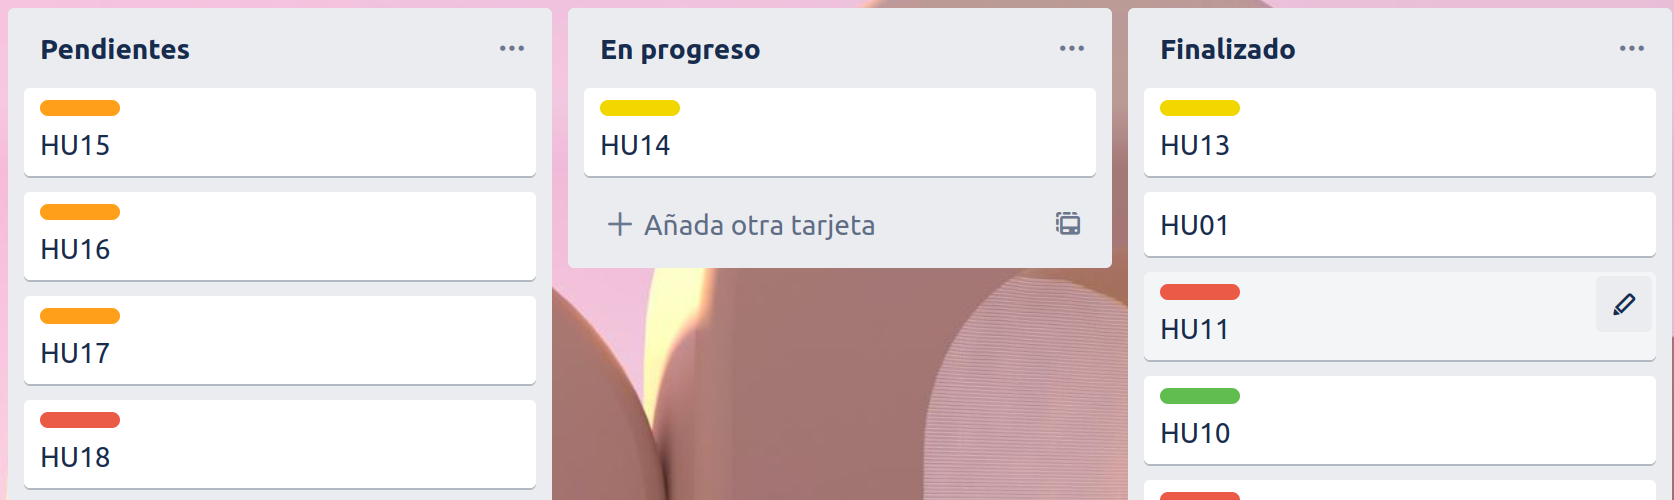
\includegraphics[width=14cm]{img/tables/09_Trello.png}
    \caption{Estado del tablero \textit{Kanban} durante el desarrollo.}
    \label{fig:trellokanban}
\end{figure}

%%%%%%%%%%%%%%%%%%%%%%%%%%%%%
%% Variations
%%%%%%%%%%%%%%%%%%%%%%%%%%%%%

\section{Desviaciones respecto a la planificación inicial} \label{sec:variations}

A lo hora de desarrollar el proyecto, se han observado algunas irregularidades en relación a los tiempos marcados en el apartado \ref{sec:initialplan}. Dichas irregularidades son comunes al realizar aplicaciones debido a que la guía temporal que ofrece la planificación inicial, aunque contemple la corrección de errores y contratiempos, se trata solamente de una valoración subjetiva de la dimensión de las tareas.\sn

A continuación se detallan las desviaciones respecto a la planificación que se han ido encontrado a lo largo del desarrollo.\sn

\subsection{Investigación inicial} \label{sub:varinvestigation}

Esta fase se consiguió completar un 400\% más rápido de lo previsto, debido a que el autor contaba con experiencia previa relativa a temas de ciberseguridad, así como sus conceptos legales, además del conocimiento sobre la existencia de herramientas similares.\n

\subsection{\textit{Sprint} 1 - Implementación de la interfaz} \label{sub:varsprint1}

Durante la implementación de la interfaz, se encontraron varios errores asociados al paradigma de programación basado en flujos de datos, que retrasaron el \textit{sprint} seis días laborables más de lo previsto (48 horas). Esto fue debido a una incompatibilidad entre el diseño y el desarrollo que obligó a tener que pausar la tarea en curso y rediseñar por completo el modelo de flujo de datos.\sn

Para compensar este imprevisto, se optó por prescindir de la creación de pruebas unitarias al comienzo de cada \textit{sprint}, reemplazándolas por pruebas manuales en paralelo con el desarrollo.\n

\subsection{Elaboración de la documentación} \label{sub:vardoc}

Por último, se decidió dedicar 4 horas más a la elaboración de este documento, durante las cuales se diseñó una plantilla haciendo uso de herramientas especializadas en la creación de documentos científicos (ver apartado \ref{sec:latex}), con el fin de mejorar la calidad de la documentación.\n

%%%%%%%%%%%%%%%%%%%%%%%%%%%%%
%% Result
%%%%%%%%%%%%%%%%%%%%%%%%%%%%%

\section{Resultado de la planificación} \label{sec:resultplan}

Tras la realización del proyecto, se ha analizado el resultado de la planificación inicial (Apartado \ref{sec:initialplan}).\sn

A pesar los imprevistos detallados en el apartado \ref{sec:variations}, la variación total del tiempo se redujo a cuatro horas de diferencia, excediendo la fecha de finalización un día más de lo previsto \tab{realplan}.\sn

\begin{table}[H]
    \begin{center}
        \begin{tabular}{| l | c | c |}
            \hline
            \textbf{Iteración} & \textbf{T. estimado} (en horas) &  \textbf{T. real} (en horas) \\
            \hline
            Investigación inicial           & 32.0 & \cellcolor{green!10} 8.0 \\ \hline
            Especificación de requisitos    & 16.0 & 16.0 \\ \hline
            Diseño del \textit{software}    & 24.0 & 24.0 \\ \hline
            \textit{Sprint} 1: Implementación de la interfaz & 80.0 & \cellcolor{red!10} 128.0 \\ \hline
            \textit{Sprint} 2: Implementación de la \textit{API} & 48.0 & \cellcolor{green!10} 40.0 \\ \hline
            \textit{Sprint} 3: Implementación de los nodos & 40.0 & \cellcolor{green!10} 32.0 \\ \hline
            \textit{Sprint} 4: Integración del sistema & 24.0 & \cellcolor{green!10} 16.0 \\ \hline
            Elaboración del documento       & 96.0 & \cellcolor{red!10} 100.0 \\ \hline
            \textbf{Total}                  & 360.0 & \cellcolor{red!10} 364.0  \\ \hline
        \end{tabular}
    \end{center}
    \caption{Estimación temporal real en comparación con la planificación inicial.}
    \label{tab:realplan}
\end{table}
\vspace{1cm}

\subsection{Diagrama de Gantt} \label{sub:realgantt}

A continuación se muestra el tiempo real dedicado mediante un cronograma \fig{realgantt}. El eje horizontal está asociado con el marco del tiempo y, el vertical, con cada una de las iteraciones. Además, también se resaltan las desviaciones respecto a la planificación inicial.\sn

\begin{figure}[H]
    \centering
    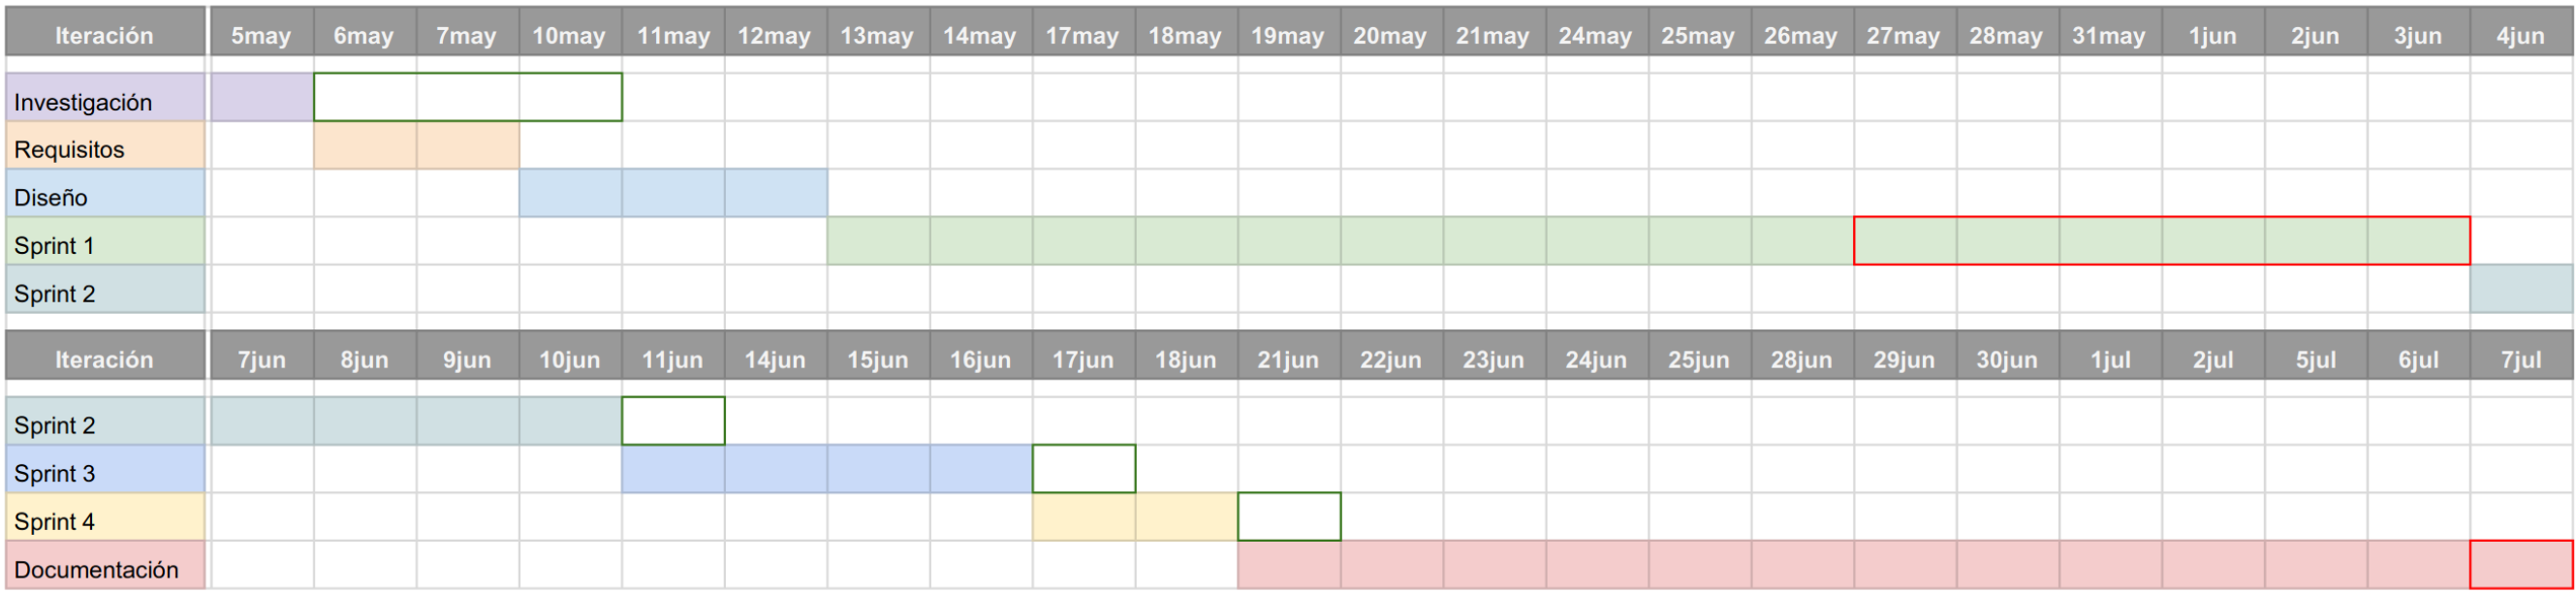
\includegraphics[width=15cm]{img/tables/10_Real-Gantt.png}
    \caption{Diagrama de Gantt resultante.}
    \label{fig:realgantt}
\end{figure}

    \blankpage
    %%%%%%%%%%%%%%%%%%%%%%%%%%%%%%%%%%%%%%%%%%%%%%%%%%%%%%%%%%%%%%%%%%
%%  ~ Trabajo de Fin de Grado - Universidad de Vigo (ESEI) ~    %%
%% Autor: Diego Enrique Fontán Lorenzo                          %%
%% Tutor: Miguel Ramón Díaz-Cacho Medina                        %%
%% Convocatoria: Julio 2020/21                                  %%
%% Título: Framework de automatización de auditorías Red Team   %%
%%%%%%%%%%%%%%%%%%%%%%%%%%%%%%%%%%%%%%%%%%%%%%%%%%%%%%%%%%%%%%%%%%

%%%%%%%%%%%%%%%%%%%%%%%%%%%%%
%% Technologies
%%%%%%%%%%%%%%%%%%%%%%%%%%%%%

\chapter{Tecnologías y lenguajes} \label{cap:tech}

En este capítulo se detallan las tecnologías y lenguajes de programación utilizados durante la realización del trabajo, así como la integración de productos de terceros, cuyo desarrollo no pertenece al autor de este documento.\sn

Ninguna de las tecnologías aquí mencionadas es vinculante al proyecto, pudiendo reemplazarse cada una de ellas por cualquiera de sus alternativas. Todas las elecciones de esta lista se han realizado valorando los conocimientos del autor, así como la comodidad durante el desarrollo.\n

%%%%%%%%%%%%%%%%%%%%%%%%%%%%%
%% Golang
%%%%%%%%%%%%%%%%%%%%%%%%%%%%%

\section{Golang} \label{sec:golang}

\footnotesize\color{gray}
\url{https://golang.org/}
\normalsize\color{black}\sn

\begin{wrapfigure}{r}{3cm}

\includegraphics[width=3cm]{img/tables/11_Golang.png}
\caption{Mascota de Golang. Gopher.}
\label{fig:golang}
\end{wrapfigure}

\textit{Golang} (o \textit{Go}) es un lenguaje de programación enfocado en la concurrencia, desarrollado por \textit{Google}. Está inspirado en la sintaxis de \textit{C}, siendo a su vez un lenguaje que cuenta con un compilador y gestor de dependencias propio. Es dinámico como \textit{Python}, pero destaca al ofrecer un rendimiento similar a \textit{C} o \textit{C++}.\sn

Será el lenguaje de programación principal del programa, encargado de levantar el servidor, manejar las peticiones \textit{HTTP} y servir los archivos estáticos.\sn

La decisión se ha llevado a cabo debido a que ofrece grandes herramientas de trabajo que permiten la ejecución de tareas concurrentes, así como las denominadas \textit{go tools}, enfocadas en proporcionar al programador la capacidad de formatear, evaluar y documentar el código, entre otras cosas. También cuenta con un compilador multiplataforma, independiente del sistema operativo y arquitectura anfitrión, con capacidad de detección de condiciones de carrera (o \textit{race conditions}), además de un gestor de paquetes integrado (similar a \textit{pip} en \textit{Python} o \textit{Gem} en \textit{Ruby}).\n

\newpage

%%%%%%%%%%%%%%%%%%%%%%%%%%%%%
%% Vue.js
%%%%%%%%%%%%%%%%%%%%%%%%%%%%%

\section{Vue.js} \label{sec:vue}

\footnotesize\color{gray}
\url{https://vuejs.org/}
\normalsize\color{black}\sn

\begin{wrapfigure}{r}{2.5cm}

\includegraphics[width=2.5cm]{img/tables/13_Vue.png}
\caption{Logo de Vue.}
\label{fig:vue}
\end{wrapfigure}

\textit{Vue} (pronunciado \textit{/vju:/}, como \textit{view}) es un \textit{framework} para construir interfaces de usuario. Se enfoca principalmente en la capa de visualización, convirtiéndose así en una elección ideal para el desarrollo de aplicaciones web del tipo \textit{Single-Page}. Además, ofrece herramientas para utilizarlo o integrarlo fácilmente con otras librerías o proyectos existentes.\sn

En este proyecto, será el encargado de manejar la interfaz de usuario.\\
En un principio se planteó el desarrollo usando \textit{React}\footnote{\textit{React} es una biblioteca \textit{Javascript} de código abierto diseñada para crear interfaces de usuario. \url{https://reactjs.org/}}, pero al final se decidió utilizar \textit{Vue} solamente con la intención de aprender a usarlo.\sn

%%%%%%%%%%%%%%%%%%%%%%%%%%%%%
%% Yarn
%%%%%%%%%%%%%%%%%%%%%%%%%%%%%

\section{Yarn} \label{sec:yarn}

\footnotesize\color{gray}
\url{https://yarnpkg.com/}
\normalsize\color{black}\sn

\begin{wrapfigure}{r}{2.5cm}

\includegraphics[width=2.5cm]{img/tables/12_Yarn.png}
\caption{Logo de Yarn.}
\label{fig:yarn}
\end{wrapfigure}

\textit{Yarn} es un instalador de módulos \textit{JavaScript} y gestor de dependencias desarrollado por \textit{Facebook}, en colaboración con otras organizaciones (como \textit{Google}). Es muy rápido y muy fácil de usar, debido a que fue concebido teniendo la seguridad y el rendimiento como objetivos prioritarios.\sn

Su integración en este proyecto ofrece comodidad al desarrollar. Se puede sustituir por \textit{npm} (su alternativa directa), o prescindir completamente del gestor de dependencias utilizando copias locales del software de terceros requerido.\sn

%%%%%%%%%%%%%%%%%%%%%%%%%%%%%
%% GNU Make
%%%%%%%%%%%%%%%%%%%%%%%%%%%%%

\section{GNU Make} \label{sec:make}

\footnotesize\color{gray}
\url{https://www.gnu.org/software/make/}
\normalsize\color{black}\sn

\begin{wrapfigure}{r}{2.55cm}

\includegraphics[width=2.55cm]{img/tables/14_GNU-Make.png}
\caption{Logo de GNU.}
\label{fig:make}
\end{wrapfigure}

\textit{Make} es una herramienta pensada en dirigir la compilación o generación automática de un proyecto. Ofrece una sintaxis propia enfocada en definir tareas con las que ejecutar los comandos necesarios para llevar a cabo el proceso de compilación.\sn

En este proyecto, proporcionará una manera automatizada de generar el programa realizando todas las tareas de compilación necesarias.\sn

%%%%%%%%%%%%%%%%%%%%%%%%%%%%%
%% Docker
%%%%%%%%%%%%%%%%%%%%%%%%%%%%%

\section{Docker} \label{sec:docker}

\footnotesize\color{gray}
\url{https://docker.com/}
\normalsize\color{black}\sn

\begin{wrapfigure}{r}{3cm}

\includegraphics[width=3cm]{img/tables/15_Docker.png}
\caption{Logo de Docker.}
\label{fig:docker}
\end{wrapfigure}

\textit{Docker} es un proyecto enfocado en automatizar el despliegue de aplicaciones dentro de contenedores. Proporcionan una capa adicional de abstracción y permite la automatización de la virtualización de aplicaciones en múltiples sistemas operativos.\sn

Su uso está reservado para poder realizar también la distribución de la aplicación final en forma de contenedor a través de un fichero \textit{Dockerfile}. Además, proporciona la opción de orquestar un entorno completo de desarrollo mediante \textit{docker-compose}.\sn

%%%%%%%%%%%%%%%%%%%%%%%%%%%%%
%% Swagger
%%%%%%%%%%%%%%%%%%%%%%%%%%%%%

\section{Swagger} \label{sec:swagger}

\footnotesize\color{gray}
\url{https://swagger.io/}
\normalsize\color{black}\sn

\begin{wrapfigure}{r}{3cm}

\includegraphics[width=3cm]{img/tables/16_Swagger.png}
\caption{Logo de Swagger.}
\label{fig:swagger}
\end{wrapfigure}

\textit{Swagger} es un conjunto de herramientas de software de código abierto para diseñar, construir, documentar, y utilizar servicios web \textit{RESTful}. Consta de una sintaxis basada en \textit{JSON} o \textit{YAML} para generar documentación automatizada tanto de código como de casos de prueba.\sn

En este proyecto, proporcionará la documentación de las llamadas relativas a la \textit{API}, así como sus requisitos, códigos de respuesta, el modelo de los parámetros y ejemplos de uso.\sn

La documentación generada no será incluida en la versión compilada debido a que se consideraría una vulnerabilidad del tipo \textit{Information Disclosure}. Además, al ser un \textit{software} de terceros, podría causar nuevos vectores de ataques contra la aplicación. 

%%%%%%%%%%%%%%%%%%%%%%%%%%%%%
%% LaTeX
%%%%%%%%%%%%%%%%%%%%%%%%%%%%%

\section{\LaTeX} \label{sec:latex}

\footnotesize\color{gray}
\url{https://latex-project.org/}
\normalsize\color{black}\sn

\begin{wrapfigure}{r}{3cm}

\includegraphics[width=3cm]{img/tables/17_LaTeX.png}
\caption{Logo de \LaTeX.}
\label{fig:latex}
\end{wrapfigure}

``\LaTeX\textbf{ }\emph{es un sistema de composición tipográfica de alta calidad. Incluye funciones diseñadas para la producción de documentación técnica y científica. Es el estándar de facto para la comunicación y publicación de documentos científicos, además de que está desarrollado bajo la ideología de software libre.''
} --\textit{Wikipedia}\sn

Es el sistema con el que está generado este documento. Su elección se debe a su gran capacidad de personalización de artículos mediante código, similar a un lenguaje de programación.\sn

%%%%%%%%%%%%%%%%%%%%%%%%%%%%%
%% Other tools
%%%%%%%%%%%%%%%%%%%%%%%%%%%%%

\section{Otras tecnologías} \label{sec:othertools}

A continuación, se describen otras tecnologías y herramientas secundarias para la realización de este proyecto:\n

\textbf{Git}: Control de versiones pensando en la eficiencia, la confiabilidad y la compatibilidad. Es un estándar para la gestión de repositorios. \color{gray}\url{https://git-scm.com/}\color{black}\n

\textbf{GitHub}: Web enfocada a alojar proyectos utilizando el sistema de control de versiones \textit{Git}. \color{gray}\url{https://github.com/}\color{black}\n

\textbf{Visual Studio Code}: Editor de código fuente. Ofrece soporte para la depuración, control de versiones, resaltado de sintaxis, finalización inteligente de código y refactorización. \color{gray}\url{https://code.visualstudio.com/}\color{black}\n

\textbf{UPX}: Empaquetador de ejecutables, portable y de alto rendimiento. Además, incluye funciones de protector de software. \color{gray}\url{https://upx.github.io/}\color{black}\n

\textbf{VMware Workstation Pro}: Hipervisor alojado para la gestión de máquinas virtuales. \color{gray}\url{https://www.vmware.com/products/workstation-pro.html}\color{black}\n

\textbf{Trello}: Tablón virtual versátil e intuitivo usado para cualquier tipo de tarea que requiera organizar información. \color{gray}\url{https://trello.com}\color{black}\n

\textbf{MockFlow}: Herramienta de \textit{wireframing}. Permite crear \textit{wireframes} y \textit{mockups} en la nube. \color{gray}\url{https://mockflow.com}\color{black}\n

\textbf{Google Sheets}: Programa de hoja de cálculo de \textit{Google} basado en la web. \color{gray}\url{https://docs.google.com/spreadsheets}\color{black}\sn

Como mención especial, se ha utilizado la librería \textbf{ReteJS} (\url{https://rete.js.org/}) para manejar el flujo de datos. Las limitaciones de la misma, como pueden ser los eventos personalizados, controles sobre el estado del editor o su correcta integración con \textit{VueJS}, han sido resueltas mediante \textit{plugins} creados por el autor de este documento.
    \blankpage
    %%%%%%%%%%%%%%%%%%%%%%%%%%%%%%%%%%%%%%%%%%%%%%%%%%%%%%%%%%%%%%%%%%
%%  ~ Trabajo de Fin de Grado - Universidad de Vigo (ESEI) ~    %%
%% Autor: Diego Enrique Fontán Lorenzo                          %%
%% Tutor: Miguel Ramón Díaz-Cacho Medina                        %%
%% Convocatoria: Julio 2020/21                                  %%
%% Título: Framework de automatización de auditorías Red Team   %%
%%%%%%%%%%%%%%%%%%%%%%%%%%%%%%%%%%%%%%%%%%%%%%%%%%%%%%%%%%%%%%%%%%

%%%%%%%%%%%%%%%%%%%%%%%%%%%%%
%% Requirements
%%%%%%%%%%%%%%%%%%%%%%%%%%%%%

\chapter{Análisis de requisitos} \label{cap:requirements}

En este capítulo se resumen los requisitos descritos en el apartado \ref{sub:requirements}, agrupándolos por funcionalidad y categoría, utilizando un lenguaje natural.\n

%%%%%%%%%%%%%%%%%%%%%%%%%%%%%
%% Functional
%%%%%%%%%%%%%%%%%%%%%%%%%%%%%

\section{Requisitos funcionales} \label{sub:funcrequirements}
\vspace{1cm}

\textbf{El sistema debe ser capaz de realizar auditorías de seguridad}\sn

Actualmente existen múltiples metodologías enfocadas a la realización de auditorías de ciberseguridad, como pueden ser \textit{OWASP WSTG} \cite{owaspwstg} o \textit{MITRE ATT\&CK} \cite{mitre}. Dichas metodologías definen una serie de controles o pruebas que deben ser llevadas a cabo por un auditor para garantizar la seguridad de los activos.\sn

La aplicación debe poder realizar tareas con el fin de garantizar el seguimiento de los controles más habituales.\sn

Las historias de usuario relativas a este requisito son: \footnotesize\color{black!90}
\textbf{HU02}, \textbf{HU04}, \textbf{HU09}, \textbf{HU13} y \textbf{HU14}.
\normalsize\color{black}\n

\textbf{El usuario podrá definir diferentes flujos de ejecución}\sn

Es importante que las tareas se realicen en un orden concreto, proporcionando al usuario los mecanismos para controlarlo, incluyendo la habilidad de establecer condiciones o de definir varios flujos de datos simultáneos.\sn

También debe ser capaz emitir eventos que inicien el flujo del programa, así como visualizar el estado actual del mismo.\sn

Las historias de usuario relativas a este requisito son: \footnotesize\color{black!90}
\textbf{HU03}, \textbf{HU06}, \textbf{HU07} y \textbf{HU08}.
\normalsize\color{black}\n

\newpage
\textbf{El sistema podrá extender su la funcionalidad mediante nuevos controles}\sn

Debido a que el mundo de la ciberseguridad está en constante cambio, es necesario que el sistema sea capaz de extenderse a través de la creación de nuevos controles sin la necesidad de cambiar el código base.\sn

Los nodos deberán estar definidos en función de una plantilla estándar que sepa interpretar la aplicación. Ésta última debe constar con un control de versiones para evitar problemas de compatibilidad.\sn

Las historias de usuario relativas a este requisito son: \footnotesize\color{black!90}
\textbf{HU05} y \textbf{HU10}.
\normalsize\color{black}\n

%%%%%%%%%%%%%%%%%%%%%%%%%%%%%
%% No-Functional
%%%%%%%%%%%%%%%%%%%%%%%%%%%%%

\section{Requisitos no funcionales} \label{sub:nofuncrequirements}
\vspace{1cm}

\textbf{El sistema debe ser intuitivo}\sn

Debe tener una interfaz amigable, para que un nuevo usuario no tarde más de un día en aprender a utilizar la aplicación.\sn

Las historias de usuario relativas a este requisito son: \footnotesize\color{black!90}
\textbf{HU01}, \textbf{HU04}, \textbf{HU15}, \textbf{HU16} y \textbf{HU17}.
\normalsize\color{black}\n

\textbf{El programa debe poder distribuirse fácimente}\sn

Es necesario que el programa sea fácil de descargar y utilizar en cualquier sistema con el fin de poder ser adoptado en entornos educativos.\sn

Las historias de usuario relativas a este requisito son: \footnotesize\color{black!90}
\textbf{HU11} y \textbf{HU12}.
\normalsize\color{black}\n

\textbf{El sistema debe contar con mecanismos de seguridad}\sn

Aunque se trate de una aplicación pensada en un uso limitado (donde el usuario la ejecute solamente cuando sea necesario), es posible valorar la idea de desplegarla sobre un servidor, dando así soporte a múltiples usuarios simultáneamente.\sn

Esto, unido a que el sistema realiza interacciones con servicios externos, requiere que se implementen ciertas medidas de seguridad que garanticen la integridad del sistema anfitrión.\sn

La historia de usuario relativa a este requisito es: \footnotesize\color{black!90}
\textbf{HU18}.
\normalsize\color{black}\n
    \blankpage
    %%%%%%%%%%%%%%%%%%%%%%%%%%%%%%%%%%%%%%%%%%%%%%%%%%%%%%%%%%%%%%%%%%
%%  ~ Trabajo de Fin de Grado - Universidad de Vigo (ESEI) ~    %%
%% Autor: Diego Enrique Fontán Lorenzo                          %%
%% Tutor: Miguel Ramón Díaz-Cacho Medina                        %%
%% Convocatoria: Julio 2020/21                                  %%
%% Título: Framework de automatización de auditorías Red Team   %%
%%%%%%%%%%%%%%%%%%%%%%%%%%%%%%%%%%%%%%%%%%%%%%%%%%%%%%%%%%%%%%%%%%

%%%%%%%%%%%%%%%%%%%%%%%%%%%%%
%% Architecture
%%%%%%%%%%%%%%%%%%%%%%%%%%%%%

\chapter{Arquitectura} \label{cap:arch}

En este capítulo se detalla la arquitectura seguida, la cual define de manera abstracta las interfaces y los componentes que llevan a cabo alguna tarea de computación, así como la comunicación entre ellos.\n

\begin{quotation}
    \textit{``La arquitectura de software se selecciona y diseña con base en objetivos (requisitos) y restricciones. Los objetivos son aquellos prefijados para el sistema de información, [...] como el mantenimiento, la auditoría, flexibilidad e interacción con otros sistemas de información. Las restricciones son aquellas limitaciones [...] derivadas de las tecnologías disponibles para implementar sistemas de información.''} -- Wikipedia.\n
\end{quotation}

Existen varios tipos de arquitecturas seguidas durante el desarrollo del proyecto. A continuación se detalla cada una de ellas y se explican los beneficios que otorgan al producto final.\n

%%%%%%%%%%%%%%%%%%%%%%%%%%%%%
%% Pipeline
%%%%%%%%%%%%%%%%%%%%%%%%%%%%%

\section{Arquitectura en \textit{pipeline}} \label{sec:pipelinarch}

%La arquitectura basada en filtros (o \textit{pipeline}) \cite{wikiPipeline} consiste en ir transformando un flujo de datos durante un proceso de etapas secuenciales (siendo la entrada de cada una la salida de la anterior) mediante el uso de filtros operacionales. Es muy común en la programación funcional, ya que equivale a la composición de funciones matemáticas.\sn

La arquitectura basada en filtros (o \textit{pipeline}) debe su nombre al uso de tuberías para procesar información. Una \textbf{tubería} es una cola de mensajes, donde un mensaje puede ser cualquier cosa. Un filtro es un proceso, hilo u otro componente que lee perpetuamente los mensajes de una tubería de entrada, uno a la vez, procesa cada mensaje y luego escribe el resultado en una tubería de salida \cite{pipelineArch}.\sn

A pesar de no ser una de las arquitecturas más populares, su uso es frecuente en el mundo de la programación. Como ejemplos, se pueden destacar los patrones que siguen el diseño \textit{map-filter-reduce} para tratamiento de listas, o el intérprete de comandos propio de cualquier sistema operativo, en el que se enlazan tareas por medio de tuberías (o \textit{pipes}).\sn

\textbf{Es la arquitectura base de este proyecto}, debido a que es uno de los principios de la programación visual y, en concreto, la programación basada en flujos de datos. Esta arquitectura es apreciable de forma gráfica mediante el editor de nodos.

%%%%%%%%%%%%%%%%%%%%%%%%%%%%%
%% Blackboard
%%%%%%%%%%%%%%%%%%%%%%%%%%%%%

\section{Arquitectura en pizarra} \label{sec:boardarch}

La arquitectura en pizarra \cite{wikiBlackboard} es un marco de trabajo de sistemas que representa un enfoque general para la resolución de problemas basados en conocimiento.\sn

Su concepto es similar a la arquitectura anterior (Apartado \ref{sec:pipelinarch}). Consta de múltiples elementos funcionales, donde cada uno está especializados en una tarea concreta. Estos elementos son conocidos como \textbf{agentes} (en este caso, los nodos). Además, existe un elemento de control denominado \textbf{pizarra} (el editor de nodos). Todos los agentes cooperan para alcanzar una meta común, si bien sus objetivos individuales no suelen estar aparentemente coordinados.\sn

Cabe destacar que no es la arquitectura que mejor detalla al sistema, dado que el comportamiento básico de cualquier agente consiste en examinar la pizarra, realizar su tarea y escribir sus conclusiones en la misma pizarra. En el caso concreto de la aplicación, los agentes interactúan directamente entre sí, aunque pueden obtener el estado de otros agentes mediante la pizarra. Esto permite, a su vez, obtener una traza de las operaciones realizadas durante el proceso de resolución.\sn

Aún así, sí que define correctamente varios aspectos del sistema: la pizarra facilita la conexión, coordinando a los distintos agentes, y los resultados generados por los agentes deben responder a un lenguaje y semántica común.\n

%%%%%%%%%%%%%%%%%%%%%%%%%%%%%
%% Services
%%%%%%%%%%%%%%%%%%%%%%%%%%%%%

\section{Arquitectura orientada a servicios} \label{sec:servicearch}

La arquitectura orientada a servicios \cite{wikiSOA} o \textit{SOA} (del inglés \textit{Service Oriented Architecture}) es un tipo de arquitectura que se basa en la creación de representaciones lógicas de ciertas actividades y que tiene un resultado de negocio específico (por ejemplo: comprobar el crédito de un cliente, obtener datos de clima, consolidar reportes de perforación, \textit{etc.}). Los \textbf{servicios}, a su vez, se definen como funciones sin estado, auto-contenidas, que aceptan una o más llamadas y devuelve una o más respuestas mediante una interfaz bien definida.\sn

En la aplicación, es la arquitectura que sigue la \textbf{API}, la cual estará formada por rutas y \textit{middlewares} que acturán como servicios.\sn


    \blankpage
    \include{sections/chapters/06_diseño}
    \blankpage
    %%%%%%%%%%%%%%%%%%%%%%%%%%%%%%%%%%%%%%%%%%%%%%%%%%%%%%%%%%%%%%%%%%
%%  ~ Trabajo de Fin de Grado - Universidad de Vigo (ESEI) ~    %%
%% Autor: Diego Enrique Fontán Lorenzo                          %%
%% Tutor: Miguel Ramón Díaz-Cacho Medina                        %%
%% Convocatoria: Julio 2020/21                                  %%
%% Título: Framework de automatización de auditorías Red Team   %%
%%%%%%%%%%%%%%%%%%%%%%%%%%%%%%%%%%%%%%%%%%%%%%%%%%%%%%%%%%%%%%%%%%

%%%%%%%%%%%%%%%%%%%%%%%%%%%%%
%% Data
%%%%%%%%%%%%%%%%%%%%%%%%%%%%%

\chapter{Gestión de los datos e información} \label{cap:data}

En este capítulo se detalla cómo se gestiona la información que maneja la aplicación. El tratamiento de estos datos se realiza de dos maneras diferentes, dependiendo de si son parte del flujo de datos perteneciente a los nodos del editor o a la \textit{API}.\n

%%%%%%%%%%%%%%%%%%%%%%%%%%%%%
%% Nodes
%%%%%%%%%%%%%%%%%%%%%%%%%%%%%

\section{Información de los nodos} \label{sec:nodedata}

Los nodos tienen tres vías principales (las entradas, las salidas y los controles) \fig{nodeskel} y una secundaria (llamadas a la \textit{API}) por las que manejan datos. Las \textbf{entradas} son la información que recibe de otros nodos; \textbf{los controles}, la información que condiciona el comportamiento del nodo y \textbf{las salidas}, la información que transmite en relación a sus entradas y/o controles. Un nodo puede estar formado por cualquier combinación de entradas, salidas y controles.\sn

\begin{figure}[H]
    \centering
    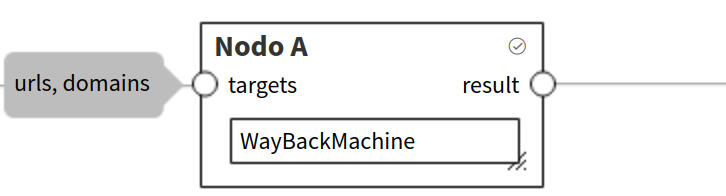
\includegraphics[width=8cm]{img/tables/26_Ingredient.png}
    \caption{Representación de un nodo.}
    \label{fig:nodeskel}
\end{figure}

Las entradas y las salidas se visualizan a modo de conectores (de izquierda a derecha, respectivamente) Las salidas pueden conectarse a las entradas mediante cables y todos los datos que se transmiten están sujetos a un modelo \textit{tipado}, similar a los tipos de variables en los lenguajes de programación tradicionales. Dos conectores con tipos de datos incompatibles no se pueden unir entre sí.\sn

Dichos tipos de datos se generan automáticamente a la par que los nodos, los cuales son especificados mediante un archivo con formato \textit{YAML\footnote{\textit{YAML Ain't Markup Language}. \url{https://yaml.org/}}\fig{ingredientspec}}. Los tipos de datos pueden comprobarse estacionando el cursor encima del conector en el que se esté interesado. Además, existe un tipo de dato, \textbf{\textit{any}}, que no tiene restricciones de conexión.\sn

Respecto a la ejecución, los nodos reportan su estado mediante un icono en la parte superior derecha.

Por otra parte, actualmente existen cuatro estilos de controles diferentes que se pueden implementar en un nodo. Los controles no son más que la abstracción de los elementos propios de formularios \textit{HTML}: \textbf{\textit{Area}}, \textbf{\textit{Check}}, \textbf{\textit{Input}} y \textbf{\textit{Options.}}\sn

\begin{figure}[H]
    \centering
    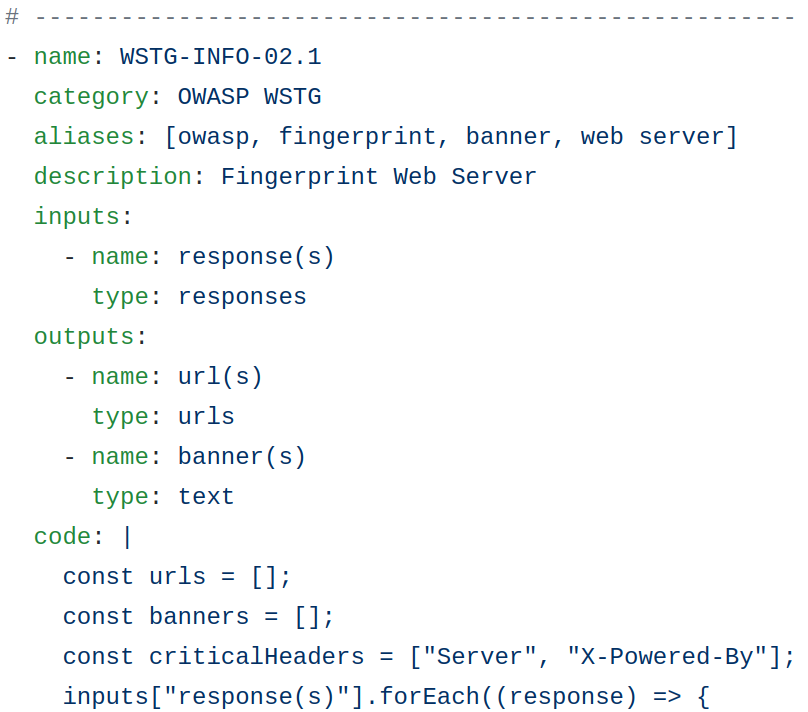
\includegraphics[width=8cm]{img/tables/27_Ingredient-Spec.png}
    \caption{Especificación de un nodo.}
    \label{fig:ingredientspec}
\end{figure}

Por último, tal como se puede observar en la figura \ref{fig:ingredientspec}, los nodos procesan los datos mediante código \textit{JavaScript}. Este código consta de cuatro variables globales principales a la hora de manejar los datos que son: \textit{inputs} (datos de entrada), \textit{outputs} (datos de salida), \textit{node.data} (parámetros de los controles) y \textit{call} (llamadas a la \textit{API} usando \textit{fetch}). Para más información, consultar en el Anexo \ref{anx:manual}.\sn

Además, para evitar bucles infinitos de procesamiento o ejecuciones innecesarias, el motor que maneja el flujo de datos comprueba si los \textit{inputs} o controles han cambiado desde la última ejecución, las entradas requeridas están conectadas y si los datos que se transmiten por ellas son válidos, evitando evaluar el código si alguna de estas condiciones no se cumple.\n

%%%%%%%%%%%%%%%%%%%%%%%%%%%%%
%% API
%%%%%%%%%%%%%%%%%%%%%%%%%%%%%

\section{Información de la \textit{API}} \label{sec:apidata}

Respecto a los datos que maneja la \textit{API} (documentado en profundidad en el Anexo \ref{anx:manual}), viajan a través del protocolo \textit{HTTP}. Al ser un servicio, se pueden realizar peticiones sin necesidad de usar el editor, lo cual permite integrar la \textit{API} en flujos de trabajos externos.\sn

Tal como se explica en el apartado \ref{sec:classdiagram}, cuando llega una petición a la \textit{API}, lo primero que hace es comprobar que tenga el formato correcto. Entre otras cosas, busca dentro de la petición la cabecera personalizada ``\textit{X-Powered-By: Masterchef!}'' y exige que la petición sea realizada usando el verbo \textit{POST}. Posteriormente, procesa los datos en el cuerpo de la petición y envía una respuesta, ambos en formato \textit{JSON}.
    \blankpage
    %%%%%%%%%%%%%%%%%%%%%%%%%%%%%%%%%%%%%%%%%%%%%%%%%%%%%%%%%%%%%%%%%%
%%  ~ Trabajo de Fin de Grado - Universidad de Vigo (ESEI) ~    %%
%% Autor: Diego Enrique Fontán Lorenzo                          %%
%% Tutor: Miguel Ramón Díaz-Cacho Medina                        %%
%% Convocatoria: Julio 2020/21                                  %%
%% Título: Framework de automatización de auditorías Red Team   %%
%%%%%%%%%%%%%%%%%%%%%%%%%%%%%%%%%%%%%%%%%%%%%%%%%%%%%%%%%%%%%%%%%%

%%%%%%%%%%%%%%%%%%%%%%%%%%%%%
%% Tests
%%%%%%%%%%%%%%%%%%%%%%%%%%%%%

\chapter{Pruebas realizadas} \label{cap:tests}

En este capítulo se detallan algunas de las pruebas llevadas a cabo durante la realización del proyecto, con el objetivo de asegurar el funcionamiento del programa, sus posibles aplicaciones en entornos reales y la correcta implementación de los requisitos descritos en el apartado \ref{cap:requirements}.\n

%%%%%%%%%%%%%%%%%%%%%%%%%%%%%
%% Disponibility
%%%%%%%%%%%%%%%%%%%%%%%%%%%%%

\section{Pruebas de disponibilidad e integridad} \label{sec:disptest}

El proyecto debe contar con la capacidad de garantizar que tanto el sistema como los datos van a estar disponibles al usuario en todo momento.\sn

Con el fin de evidenciar este aspecto, se han realizado \textbf{pruebas de estrés} y \textbf{de rendimiento}.\sn

\large
\textbf{Pruebas de estrés y rendimiento}\sn
\normalsize

Consisten en medir la capacidad del sistema en función a la carga de trabajo y sus tiempos de respuesta. Este tipo de pruebas \textbf{dependen de las especificaciones del sistema operativo anfitrión}, sus procesos y la calidad de la conexión a Internet\footnote{Pruebas realizadas sobre Ubuntu 20.04 con 8Gb de RAM, 2Gb de \textit{swap}, procesador Intel Core-i7 8th Gen y conexión por wifi (72Mbps descarga/89Mbps subida).}.\sn

Respecto al rendimiento, se ha realizado un \textit{benchmarking} mediante el uso de la herramienta \textbf{\textit{go-wrk}}\footnote{\url{https://github.com/tsliwowicz/go-wrk}}. A pesar de que \textit{Golang} cuenta con herramientas nativas de \textit{profiling}, no ofrece un buen soporte para realizar este tipo de pruebas sobre servicios \textit{HTTP}.\sn

Se han realizado tres pruebas de estrés en las que se pide a la \textit{\textbf{API}} que interaccione con una, dos y cuatrocientas páginas web reales, respectivamente. La capacidad y los tiempos de respuesta medidos durante 10 segundos son los mostrados en las figuras \ref{fig:benchAPI1URL} y \ref{fig:benchAPI2URL}. La última prueba no ha pasado el control debido a que una única petición a cuatrocientas \textit{URLs} simultáneas tarda aproximadamente medio minuto (\textit{Figs. \ref{fig:benchAPI400URL} y \ref{fig:API400URL}}).\sn

\begin{figure}[H]
    \centering
    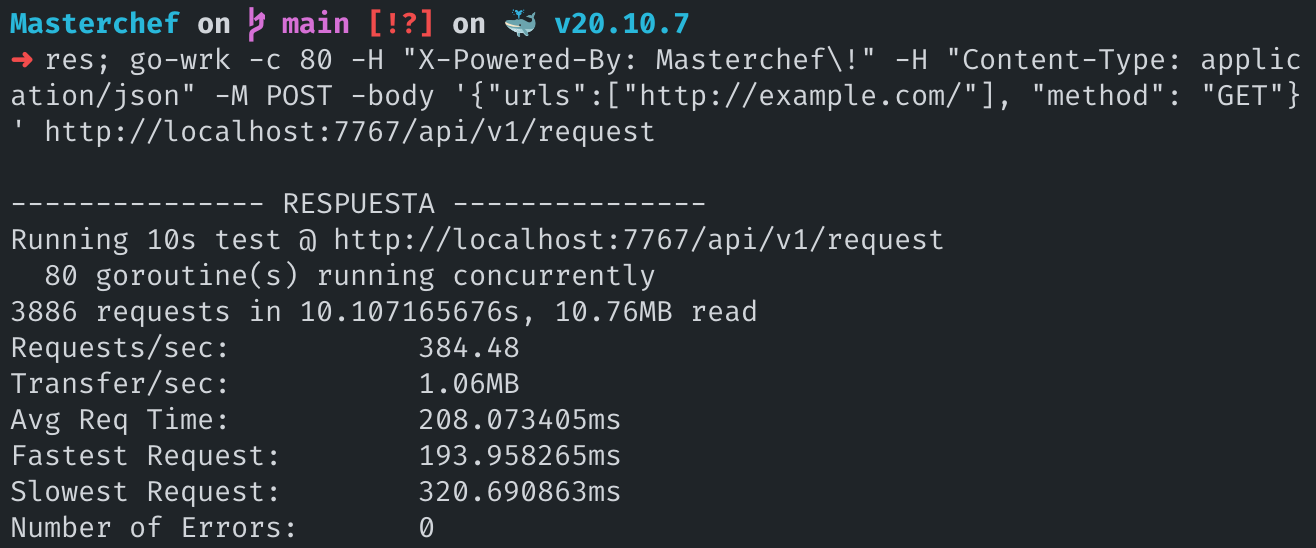
\includegraphics[width=13cm]{img/tables/28_Bench-API-1URL.png}
    \caption{\textit{Benchmark}: 3886 peticiones a 1 \textit{URL}. ~208ms/respuesta. 0 errores.}
    \label{fig:benchAPI1URL}
\end{figure}

\begin{figure}[H]
    \centering
    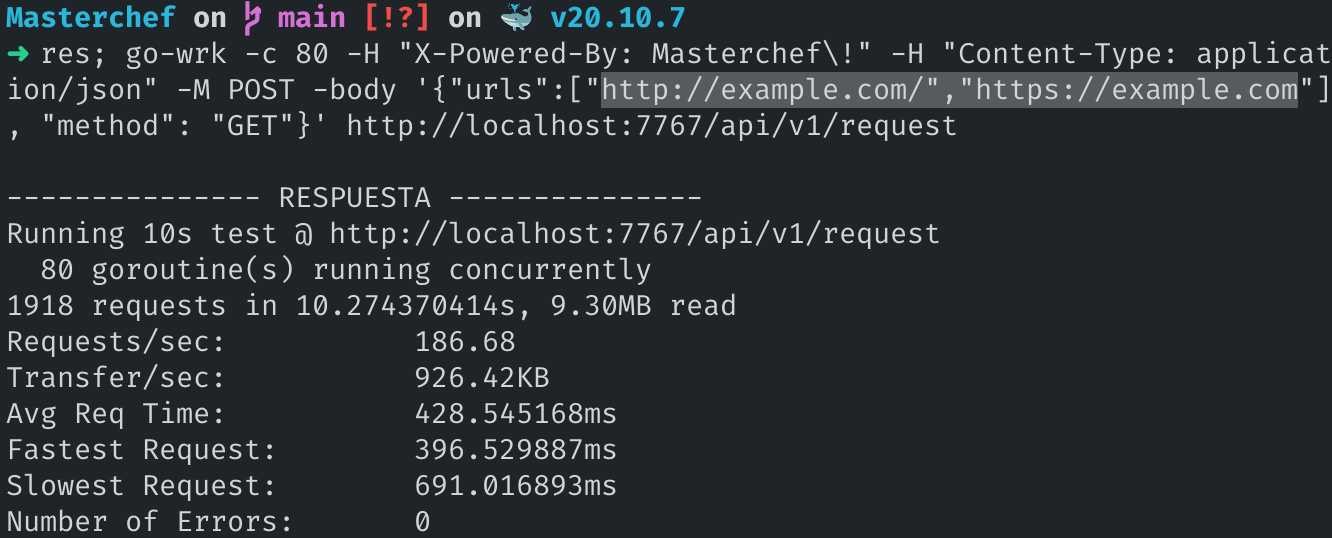
\includegraphics[width=13cm]{img/tables/29_Bench-API-2URL.png}
    \caption{\textit{Benchmark}: 1918 peticiones a 2 \textit{URLs} simultáneas. ~428ms/respuesta. 0 errores.}
    \label{fig:benchAPI2URL}
\end{figure}

\begin{figure}[H]
    \centering
    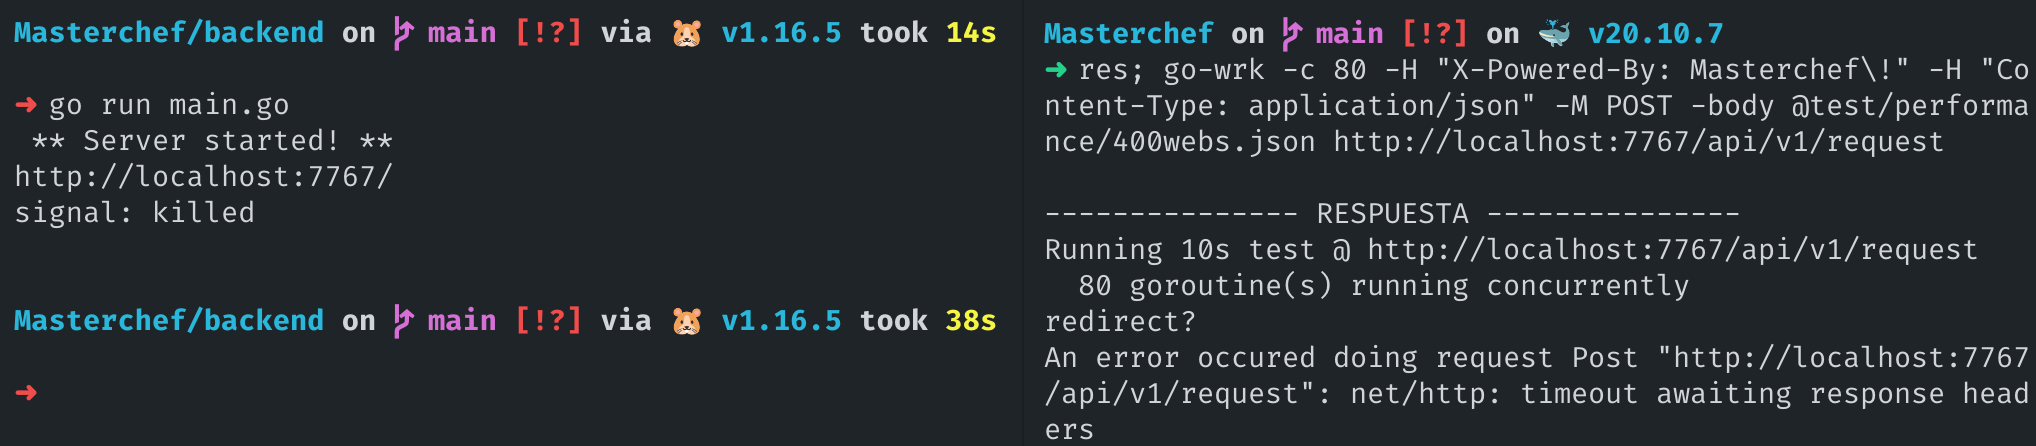
\includegraphics[width=15cm]{img/tables/31_Bench-API-400URL.png}
    \caption{\textit{Benchmark}: Peticiones a 400 \textit{URLs} simultáneas. Prueba de estrés fallida.}
    \label{fig:benchAPI400URL}
\end{figure}

\begin{figure}[H]
    \centering
    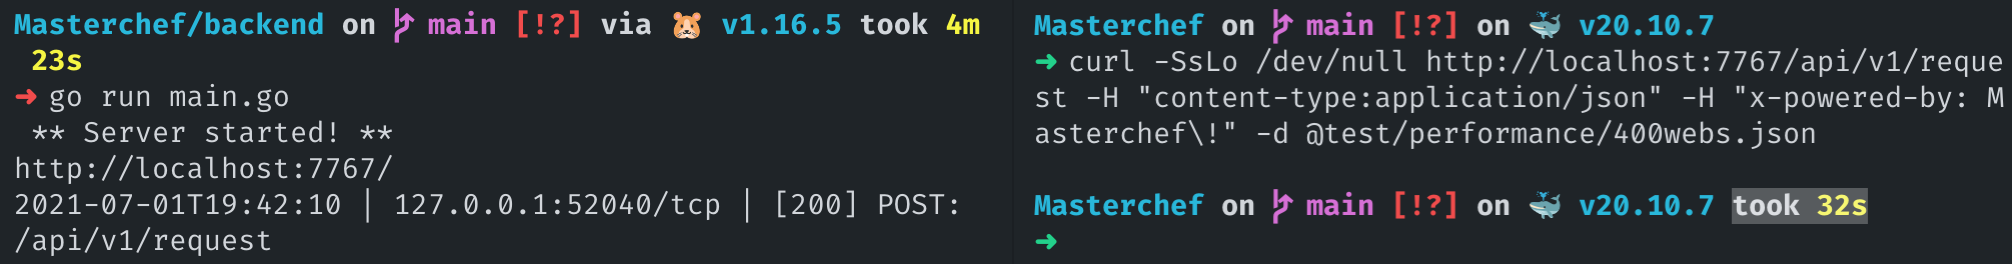
\includegraphics[width=15cm]{img/tables/32_Request-API-400URL.png}
    \caption{\textit{Test}: Petición a 400 \textit{URLs} simultáneas. ~32s/respuesta. 0 errores.}
    \label{fig:API400URL}
\end{figure}

%%%%%%%%%%%%%%%%%%%%%%%%%%%%%
%% Functionality
%%%%%%%%%%%%%%%%%%%%%%%%%%%%%

\section{Pruebas sobre la funcionalidad} \label{sec:functest}

Para comprobar la correcta funcionalidad del sistema, se han ejecutado varios tipos de flujos de datos. Estas pruebas garantizan que se cumplen los requisitos funcionales descritos en el apartado \ref{sub:funcrequirements}.\sn

La figura \ref{fig:multiplerecipe} muestra la capacidad de poder crear conjuntos de tareas independientes entre sí, así como la posibilidad de definir múltiples objetivos.\sn

\begin{figure}[H]
    \centering
    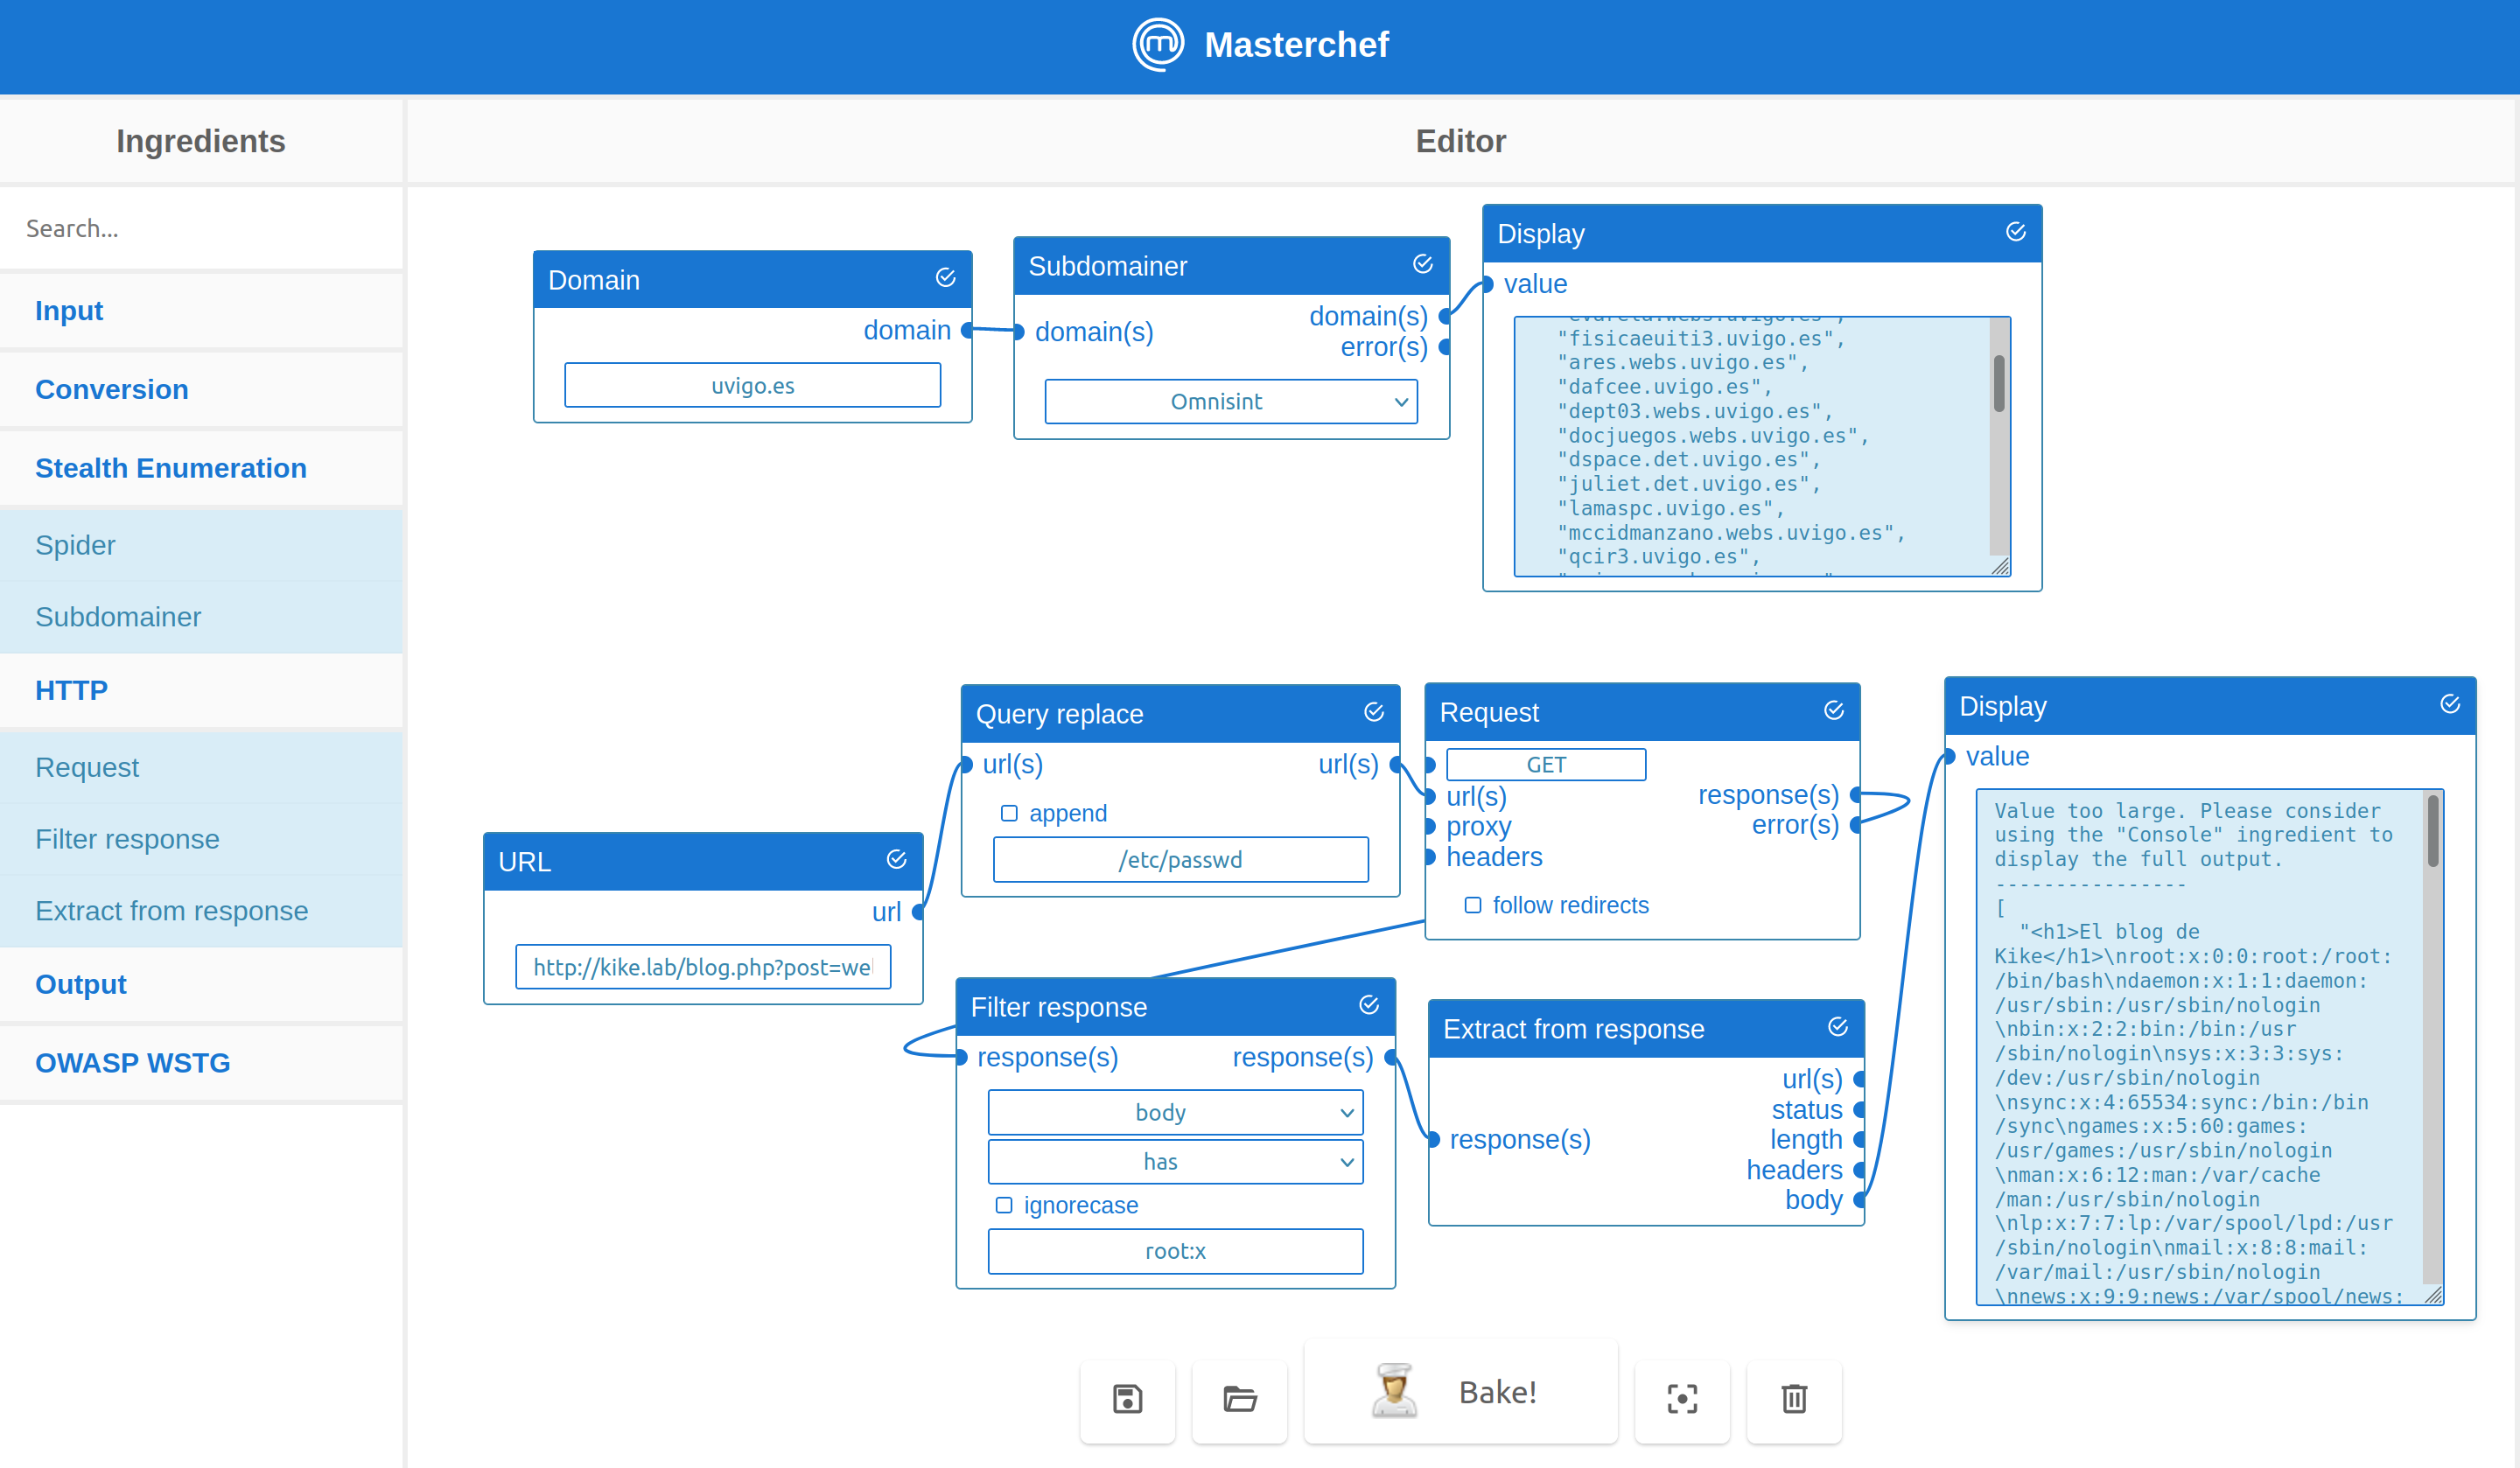
\includegraphics[width=13cm]{img/tables/33_Recipe-Multiple.png}
    \caption{Flujos independientes: Reconocimiento (arriba) y vulnerabilidad (abajo).}
    \label{fig:multiplerecipe}
\end{figure}

Además, en la figura \ref{fig:owasprecipe} se muestra cómo es posible realizar controles propios de una auditoría (ver Anexo \ref{anx:owasp}) a partir de un activo.\sn

\begin{figure}[H]
    \centering
    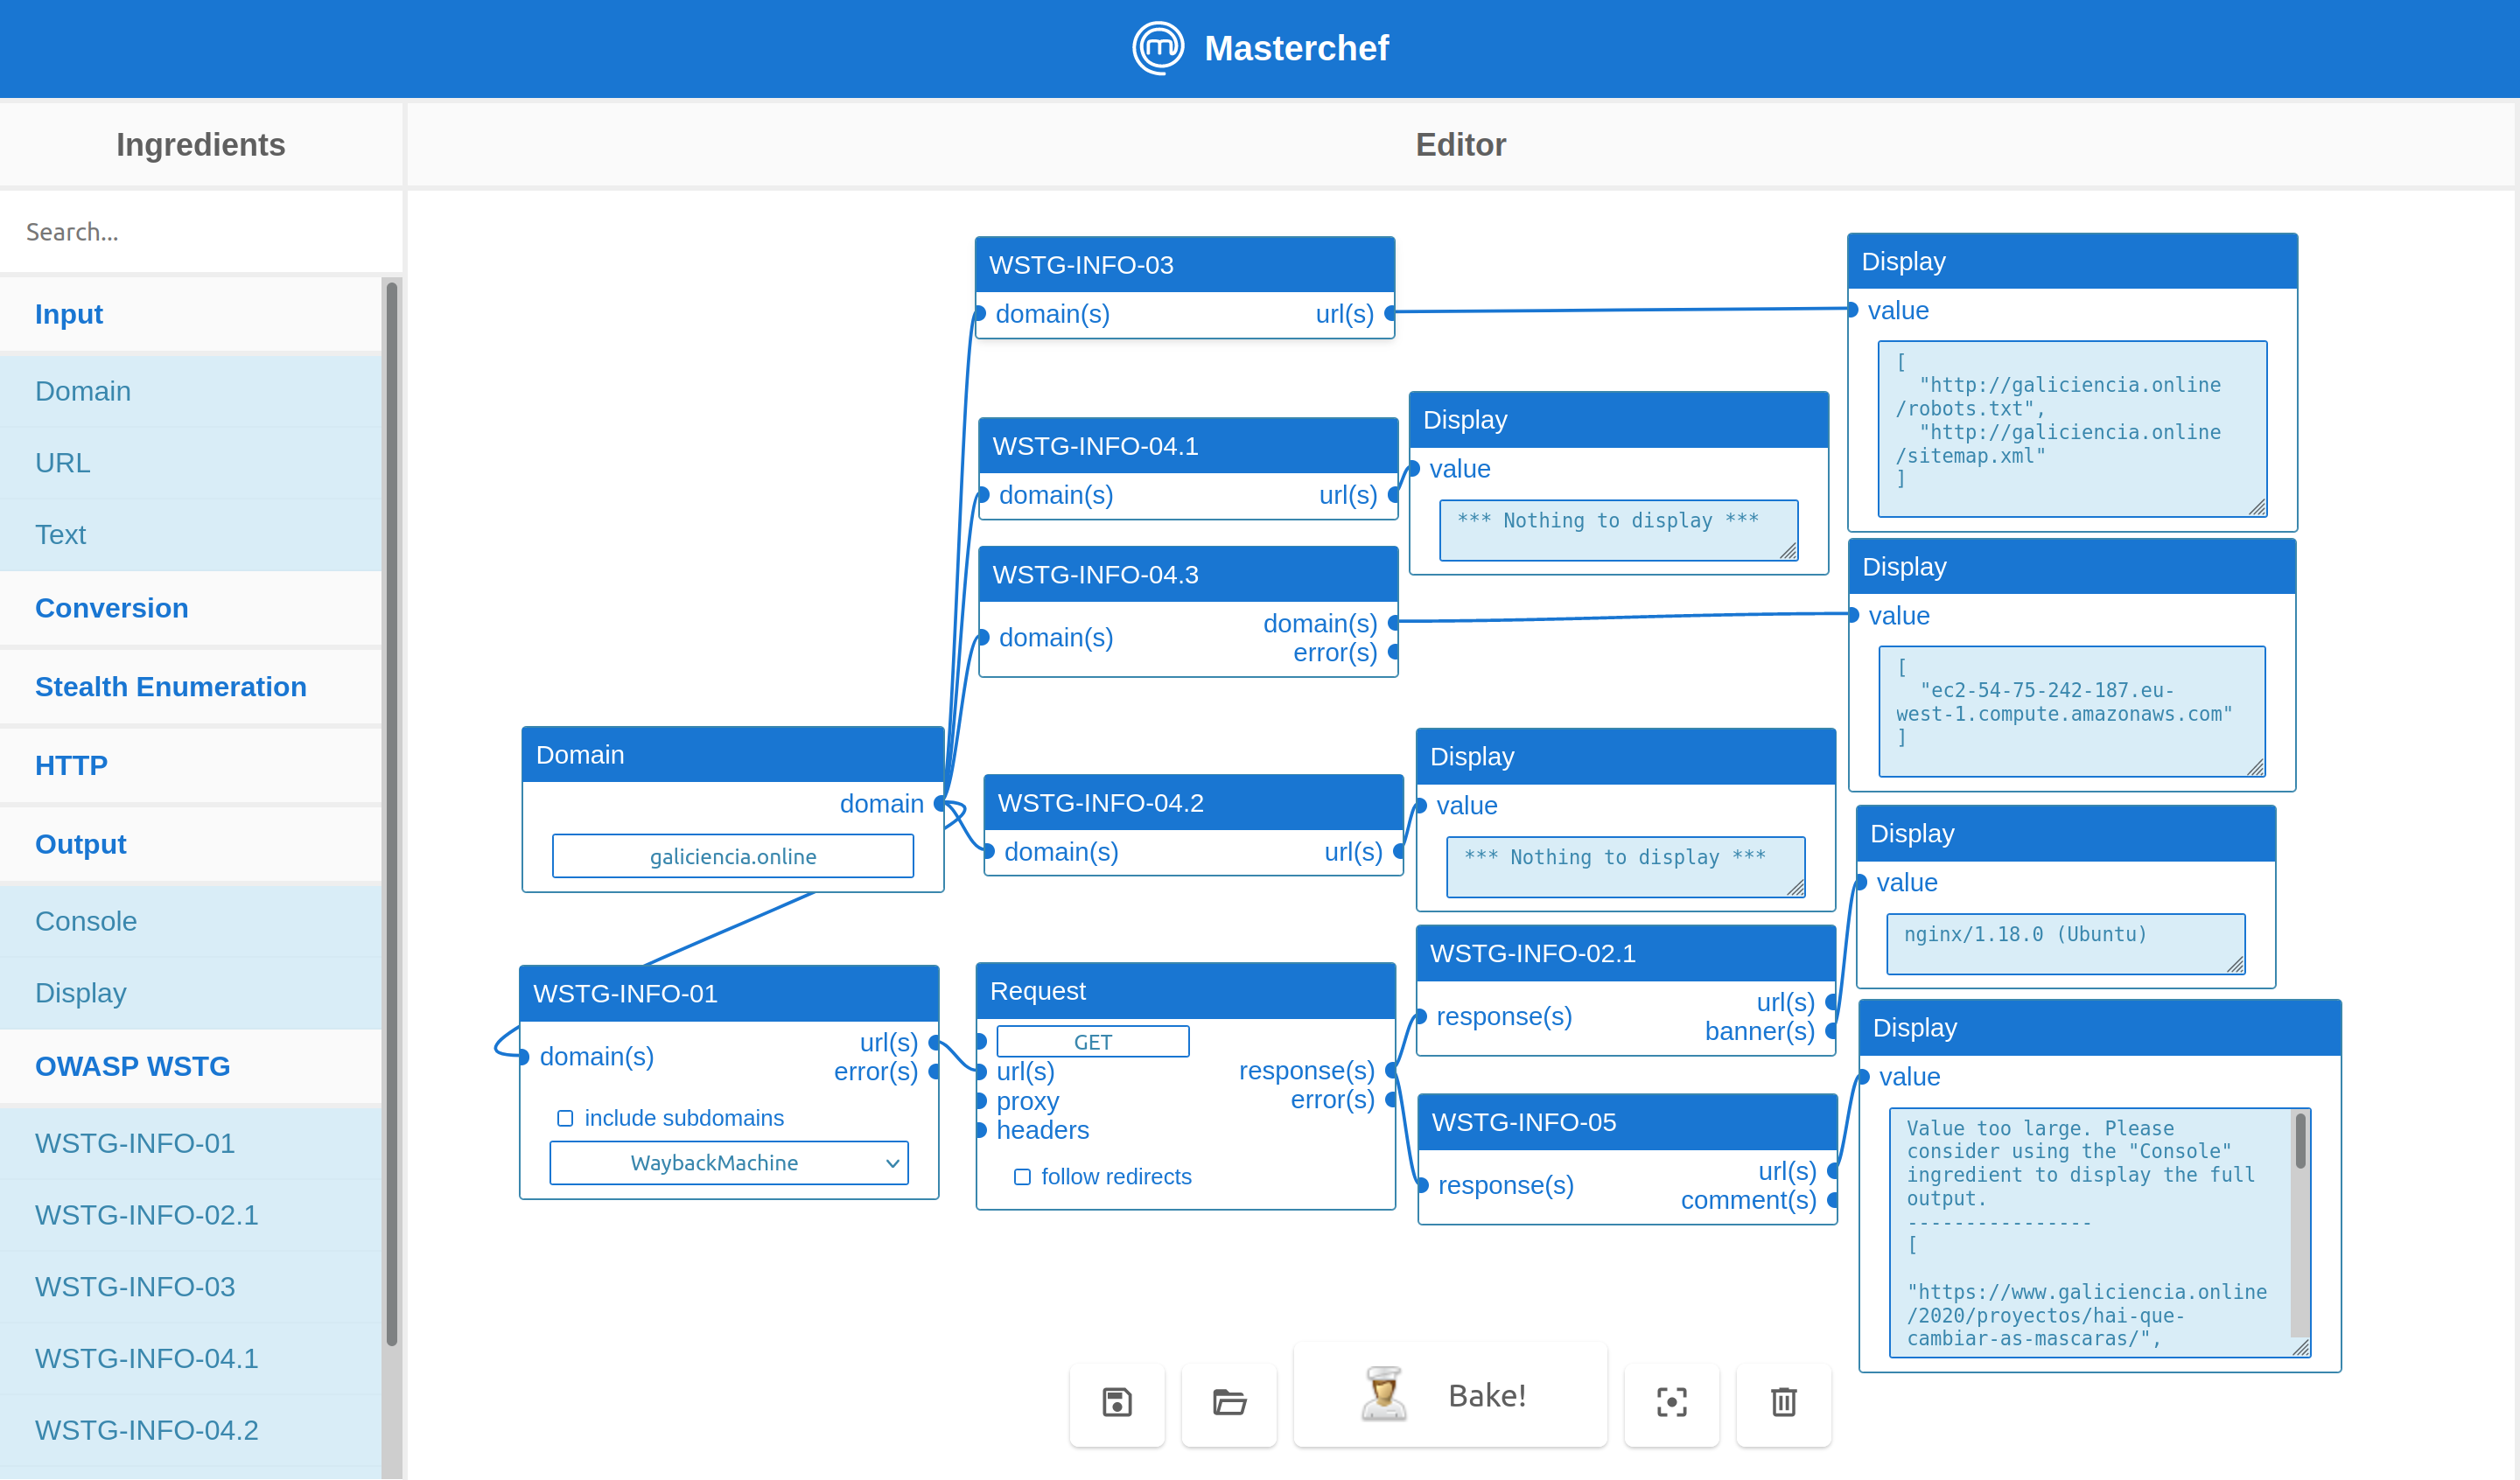
\includegraphics[width=13cm]{img/tables/34_Recipe-WSTG.png}
    \caption{Ejemplo de controles pertenecientes a \textit{OWASP WSTG-INFO}.}
    \label{fig:owasprecipe}
\end{figure}

%%%%%%%%%%%%%%%%%%%%%%%%%%%%%
%% Security
%%%%%%%%%%%%%%%%%%%%%%%%%%%%%

\section{Pruebas de seguridad} \label{sec:securitytest}

Por último, se han realizado pruebas de seguridad para garantizar la ausencia de vectores de ataques que puedan poner en peligro el sistema.\sn

Relativo al editor de nodos, las pruebas constan de la correcta gestión de errores, como bucles infinitos, que podrían provocar una sobrecarga de la \textit{CPU} \fig{reciperr}.

\begin{figure}[H]
    \centering
    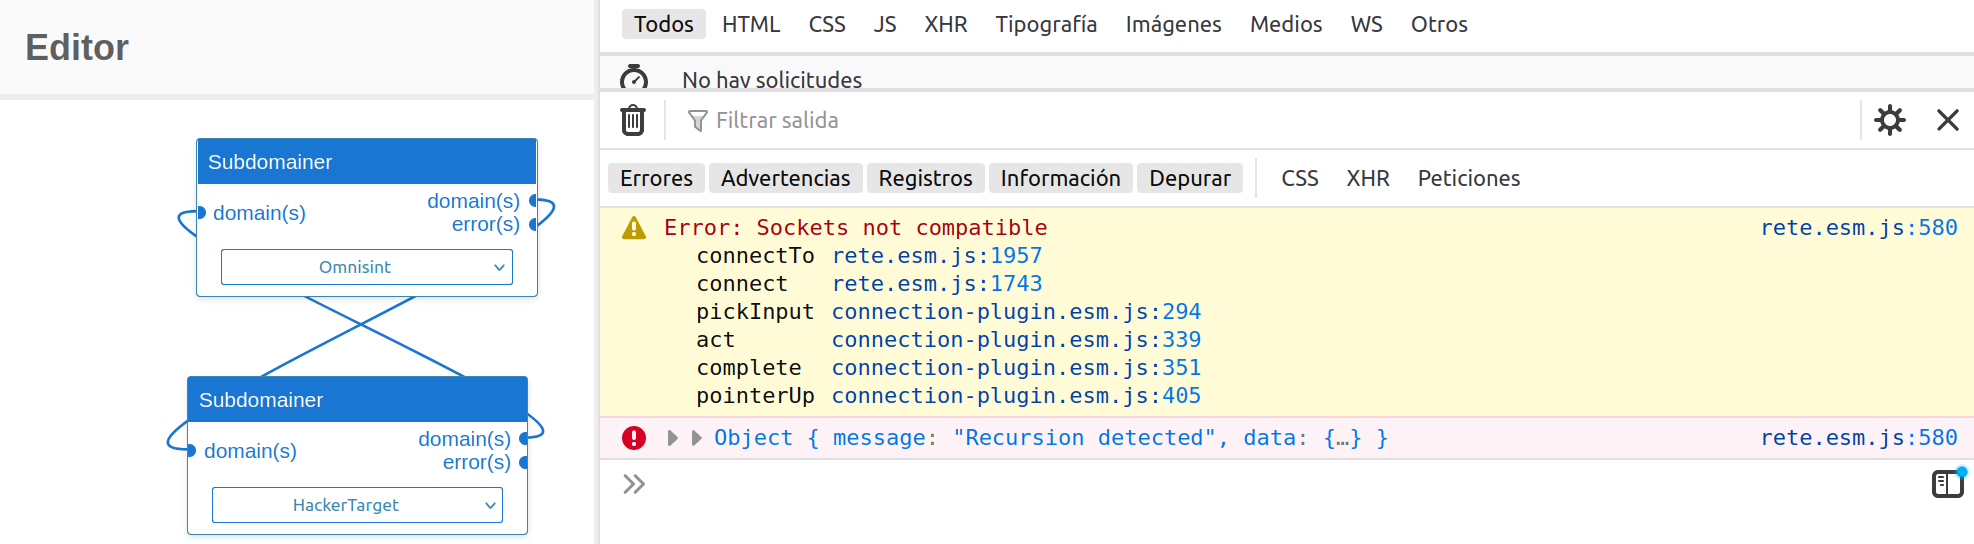
\includegraphics[width=14cm]{img/tables/35_Recipe-Errors.png}
    \caption{Manejo de errores: Conexiones incompatibles y bucles infinitos.}
    \label{fig:reciperr}
\end{figure}

Por otro lado, se han implementado medidas de seguridad para evitar los ataques web más comunes, como \textit{XSS} o \textit{Clickjacking}, mediante el uso de etiquetas \textit{span}\footnote{Las etiquetas \textit{span} no permiten la renderización de código \textit{HTML}} y cabeceras de seguridad \fig{securityrecipe}.\sn

\begin{figure}[H]
    \centering
    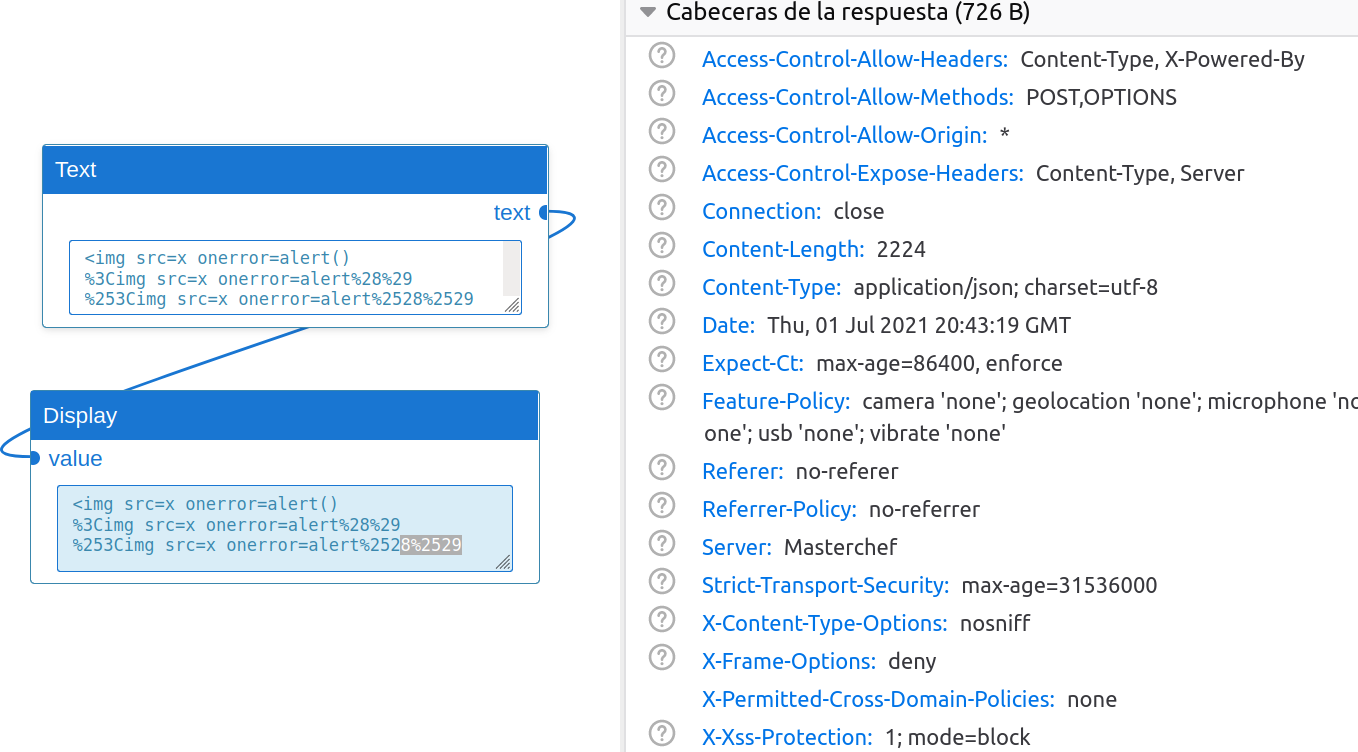
\includegraphics[width=14cm]{img/tables/36_Security.png}
    \caption{Cabeceras de seguridad y pruebas contra \textit{XSS}.}
    \label{fig:securityrecipe}
\end{figure}

Por último, el servidor se interrumpe cuando detecta peticiones más grandes de lo normal contra la \textit{API} \fig{benchAPI400URL}. Esto no se trata de una medida de seguridad, sino de una gestión de errores temporal que tendrá que ser reemplazada por medidas reales, como la segmentación de las peticiones o la implementación de listas negras.\n
    \blankpage
    \include{sections/chapters/09_epílogo}
    % appendix
    \appendix
    \blankpage
    \stepcounter{page}
    \addcontentsline{toc}{chapter}{A. Bibliografía}
    \renewcommand\bibname{A\hspace{20pt}|\hspace{20pt}Bibliografía}
    \printbibliography \label{anx:bib}
    \stepcounter{chapter}
    \blankpage
    \fancyhead[RE]{\thechapter\hspace{20pt}|\hspace{20pt}MANUAL DE USUARIO}
    %%%%%%%%%%%%%%%%%%%%%%%%%%%%%%%%%%%%%%%%%%%%%%%%%%%%%%%%%%%%%%%%%%
%%  ~ Trabajo de Fin de Grado - Universidad de Vigo (ESEI) ~    %%
%% Autor: Diego Enrique Fontán Lorenzo                          %%
%% Tutor: Miguel Ramón Díaz-Cacho Medina                        %%
%% Convocatoria: Julio 2020/21                                  %%
%% Título: Framework de automatización de auditorías Red Team   %%
%%%%%%%%%%%%%%%%%%%%%%%%%%%%%%%%%%%%%%%%%%%%%%%%%%%%%%%%%%%%%%%%%%

%%%%%%%%%%%%%%%%%%%%%%%%%%%%%
%% User guide
%%%%%%%%%%%%%%%%%%%%%%%%%%%%%

\chapter{Manual de usuario} \label{anx:manual}

En este anexo se describen los aspectos básicos de la aplicación, como la estructura de los directorios, la guía de instalación, la creación de \textit{ingredientes} y el uso básico de la misma.\sn

El código de la aplicación está disponible \textit{online} en la siguiente dirección web:\sn

\hfil\url{https://github.com/cosasdepuma/Masterchef}\hfil\n

\section{Estructura de los directorios} \label{sec:folderstructure}

Los archivos y directorios más relevantes del proyecto se encuentran estructurados siguiendo el esquema mostrado a continuación.\sn

\subsection{Directorio raíz} \label{sub:rootdir}

El \textbf{directorio raíz} cuenta con tres carpetas:\sn

\textbf{.github/}: Archivos pertenecientes a la documentación de \textit{GitHub}.

\textbf{backend/}: Código fuente del servidor.

\textbf{frontend/}: Código fuente de la interfaz.\sn

También cuenta con los siguientes ficheros:\sn

\textbf{.gitignore}: Archivos ignorados por \textit{GitHub}.

\textbf{.dockerignore}: Archivos ignorados por \textit{Docker}.

\textbf{Makefile}: Parámetros de auto-compilación.

\textbf{Dockerfile}: Archivo para compilar y desplegar la aplicación usando contenedores.

\textbf{docker-compose.yml}: Fichero para orquestar contenedores.

\textbf{version}: Versión actual del programa.

\textbf{swagger.yml}: Documentación de la \textit{API}.

\textbf{README.md}: Documentación del repositorio.

\textbf{LICENSE}: Licencia del repositorio.\sn

\subsection{Directorio \textit{frontend}} \label{sub:frontenddir}.

La carpeta \textit{frontend} cuenta con los siguientes archivos:\sn

\textbf{.browserslistrc}: Navegadores soportados por la interfaz.

\textbf{babel.config.js}: Archivo de configuración de \textit{Babel}.

\textbf{compile.js}: \textit{Script} para añadir el \textit{frontend} en ficheros \textit{.go}.

\textbf{package.json}: Archivo de configuración del \textit{frontend}.

\textbf{patches.js}: \textit{Script} para corregir errores en las dependencias.

\textbf{vue.config.js}: Archivo de configuración de \textit{Vue}.

\textbf{yarn.lock}: Versiones e integridad de las dependencias de desarrollo.\sn

Respecto a las carpetas, existen dos dentro del directorio \textit{frontend}: \textbf{public/} (con los archivos estáticos, como la plantilla \textit{HTML}) y \textbf{src/}, con el código fuente relativo al núcleo de la interfaz. Esta última está estructurada de la siguiente manera:\sn

\textbf{App.vue}: Vista principal de la aplicación.

\textbf{main.js}: Entrada de la aplicación, encargada de montar la vista.

\textbf{assets/}: Archivos auxiliares. Contiene las especificaciones de los nodos.

\textbf{components/}: Componentes visuales de la interfaz.

\textbf{ingredients/}: Archivos relativos a la interpretación de los nodos.

\textbf{scripts/}: Otros ficheros de \textit{Javascript}. Contiene la lógica del \textbf{editor/}, formado a su vez por \textbf{plugins/} y \textbf{components/} (tipos de controles). También provee de funciones auxiliares (\textbf{helpers/}), iconos (\textbf{icons/}) y validaciones (\textbf{validator/}).

\subsection{Directorio \textit{backend}} \label{sub:backenddir}.

La carpeta \textit{backend} contiene los siguientes directorios y archivos:\sn

\textbf{go.mod}: Dependencias de desarrollo.

\textbf{go.sum}: Versiones e integridad de las dependencias de desarrollo.

\textbf{main.go}: Punto de entrada de la aplicación si se ejecuta mediante un binario.

\textbf{cmd/}: Punto de entrada de la aplicación si se instala con \textit{go get}.

\textbf{public/}: Archivo auto-generados por el \textit{frontend}.

\textbf{app/}: Código fuente relativo al núcleo del servidor.\sn

La carpeta \textbf{app/} está estructurada de la siguiente forma:\sn

\textbf{config/}: Parámetros de configuración por defecto y variables de entorno.

\textbf{helpers/}: Funciones auxiliares.

\textbf{providers/}: Código para la obtención de información mediante fuentes abiertas.

\textbf{server/}: Archivos relativos al servidor \textit{HTTP}.\sn

La carpeta \textbf{server/} consta, a su vez, de los archivos \textbf{server.go} (servicio \textit{HTTP}) y \textbf{router.go} (enrutador). También cuenta con los directorios \textbf{client/} (cliente \textit{HTTP}), \textbf{middlewares/} (funciones auxiliares del enrutador) y \textbf{routes/} (rutas de la \textit{API}).\n

\section{Compilación} \label{sec:compilation}

En entornos \textit{*nix}, la compilación se puede llevar a cabo por medio del comando \textbf{make}, gracias a las reglas descritas en el archivo \textit{Makefile}.\sn

Por el contrario, si se desea realizar una compilación manual o no se dispone de las herramientas necesarias para ejecutarla de manera automatizada, se puede realizar el siguiente procedimiento:\sn

\begin{quote}
----- Interfaz

yarn --cwd frontend/ install

yarn --cwd frontend/ run compile

----- Servidor

cd backend/

go build main.go

----- Opcional

upx -o masterchef main\n
\end{quote}

\section{Instalación} \label{sec:installation}

La aplicación está disponible de modo portable. Se puede descargar directamente desde el apartado \textit{Releases} del repositorio \textit{online}. Su tamaño aproximado es de 1,9M para la versión 0.1.0.\sn

Si se desea instalar, es posible realizarlo mediante el comando\footnote{Es necesario tener \textit{Golang 1.16} instalado en el sistema}:\sn

\hfil go get -u github.com/cosasdepuma/Masterchef \hfil\n

\section{Requisitos mínimos} \label{sec:minimumrequirements}

La aplicación no cuenta con requisitos mínimos. Es posible compilarla para cualquier sistema operativo y arquitectura. Tampoco depende de ficheros o programas de terceros.\sn

En el caso de ejecutar tareas de recopilación de información o que tengan como objetivo un activo externo, puede ser necesaria una conexión a Internet.\sn

\textbf{Nota}: Actualmente el editor de nodos no funciona correctamente en dispositivos móviles o \textit{tablets}.\n

\section{Uso de la aplicación} \label{sec:usage}

A continuación, se detalla el uso de la aplicación. Se divide en tres partes: ejecución, llamadas a la \textit{API} y creación de nuevos nodos.\n

\subsection{Ejecución} \label{sub:execution}

Para iniciar el servidor, solamente basta con lanzar el programa \fig{execdefault}. Si se ejecuta desde una terminal, se pueden configurar los parámetros mediante las variables de entorno \textbf{MC\_ADDR} y \textbf{MC\_THREADS} \fig{execenv}:\sn

\begin{figure}[H]
     \centering
     \begin{subfigure}[b]{0.3\textwidth}
         \centering
         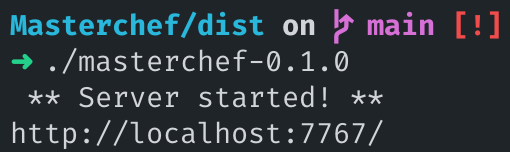
\includegraphics[width=\textwidth]{img/tables/38_Running.png}
         \caption{Ejecución estándar.}
         \label{fig:execdefault}
     \end{subfigure}
     \begin{subfigure}[b]{0.6\textwidth}
         \centering
         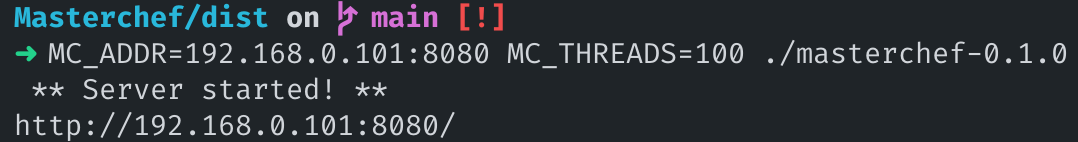
\includegraphics[width=\textwidth]{img/tables/39_Running-Env.png}
         \caption{Ejecución personalizada.}
         \label{fig:execenv}
     \end{subfigure}
    \caption{Ejecución de la aplicación.}
    \label{fig:exec}
\end{figure}

También es posible levantar el servicio usando \textit{Docker} gracias al archivo \textit{Dockerfile}.\sn

Una vez ejecutado, será necesario acceder a la dirección definida con el fin de visualizar la interfaz gráfica \fig{justtheinterface}. La \textit{URL} por defecto es \url{http://127.0.0.1:7767/}.\sn

\begin{figure}[H]
    \centering
    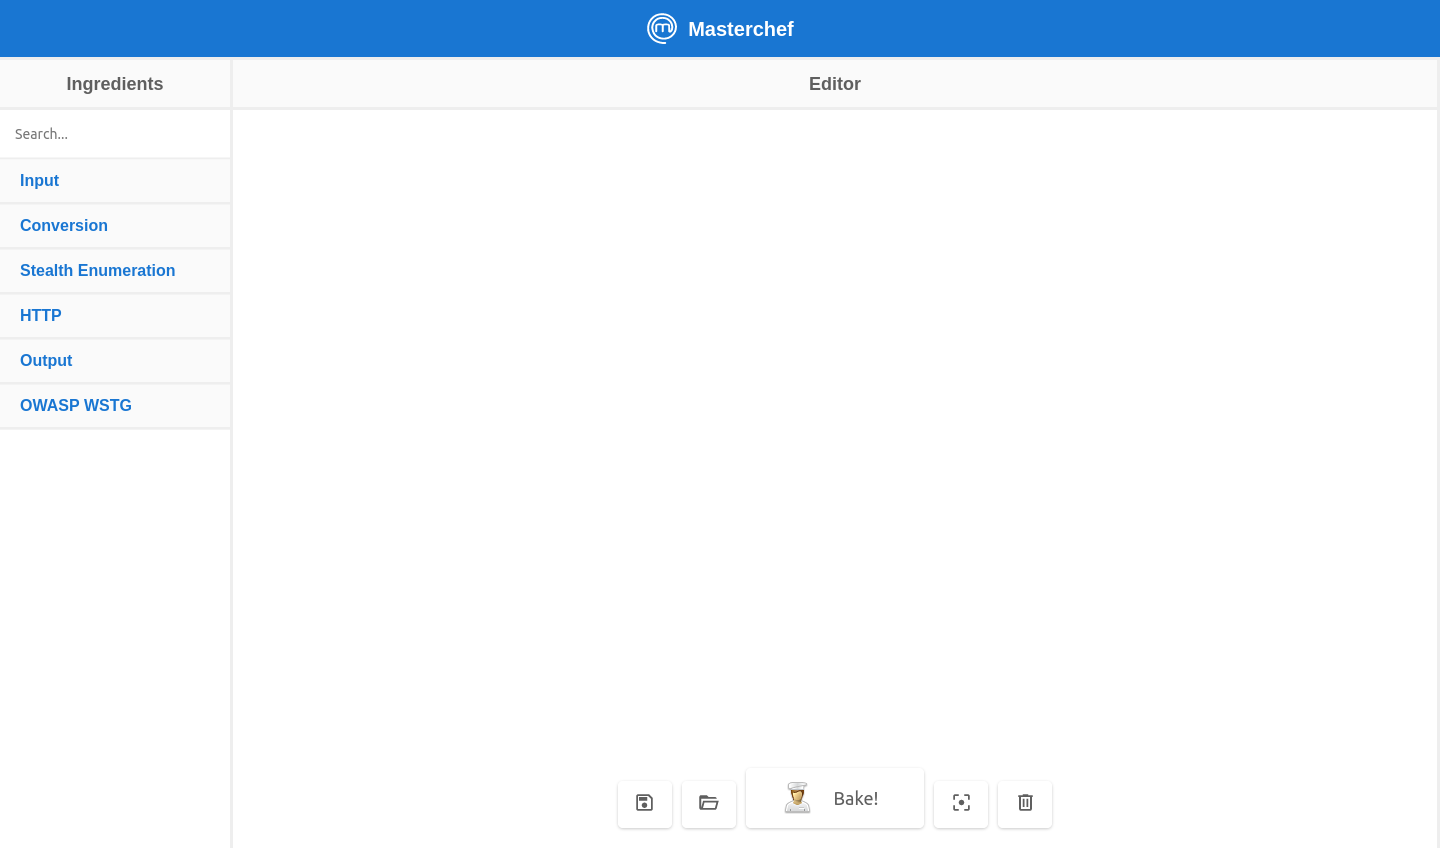
\includegraphics[width=15cm]{img/tables/40_Interface.png}
    \caption{Interfaz de la aplicación.}
    \label{fig:justtheinterface}
\end{figure}

El panel lateral izquierdo cuenta con los nodos disponibles (denominados \textit{ingredientes}). Están agrupados por categorías. Se puede desplegar u ocultar una categoría pulsando sobre ella. También contiene un buscador que permite filtrar los nodos por palabras clave. Es posible obtener la descripción de un ingrediente depositando el cursor encima del mismo \fig{ingrdesc}.\sn

\begin{figure}[H]
    \centering
    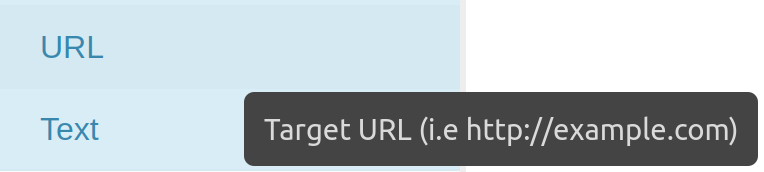
\includegraphics[width=10cm]{img/tables/41_Ingredient-Tooltip.png}
    \caption{Descripción del ingrediente.}
    \label{fig:ingrdesc}
\end{figure}

Los ingredientes pueden ser añadidos al editor arrastrándolos sobre él. Éstos constan de tres partes fundamentales \fig{ingredientskeleton}: los datos de entrada (a la izquierda), los datos de salida (a la derecha) y los controles (en el centro). Cada dato lleva asociado un tipo específico que limita su conexión con otros nodos. Para comprobar el tipo de conexión, basta con mantener el cursor encima del conector.\sn

\begin{figure}[H]
    \centering
    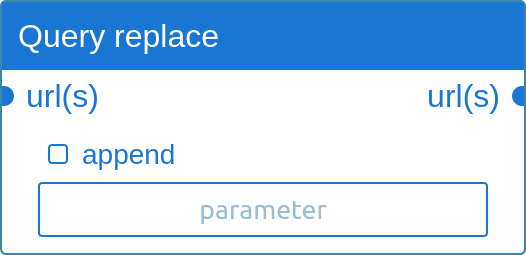
\includegraphics[width=8cm]{img/tables/42_Ingredient.png}
    \caption{Estructura de un ingrediente.}
    \label{fig:ingredientskeleton}
\end{figure}

La unión de dos o más nodos puede efectuarse arrastrando un conector de salida a uno de entrada del mismo tipo, o viceversa. Para eliminar una conexión, es posible hacerlo añadiendo una nueva o arrastrando a un espacio vacío el conector de entrada. Además, es posible eliminar un nodo pulsando la tecla \textit{Suprimir}.\sn

El editor puede controlarse mediante los botones situados en la parte inferior de la interfaz. Sus funcionalidades son, de izquierda a derecha: guardar estado actual del editor en una receta, cargar una receta desde un archivo, ejecutar el programa, centrar la vista en los nodos existentes y limpiar el editor de nodos.\sn

Cuando se ejecutan los ingredientes, es posible conocer su estado mediante un icono situado en la parte superior derecha de los mismos. Un \textit{tick} significa que el nodo se ha ejecutado correctamente; una cruz, que ha habido algún fallo (revisar la consola) y la ausencia de iconos indica que aún no ha sido procesado.\sn

\newpage

Un ejemplo de receta para buscar o comprobar vulnerabilidades puede ser la mostrada en la figura \ref{fig:openredirect}.

\begin{figure}[H]
    \centering
    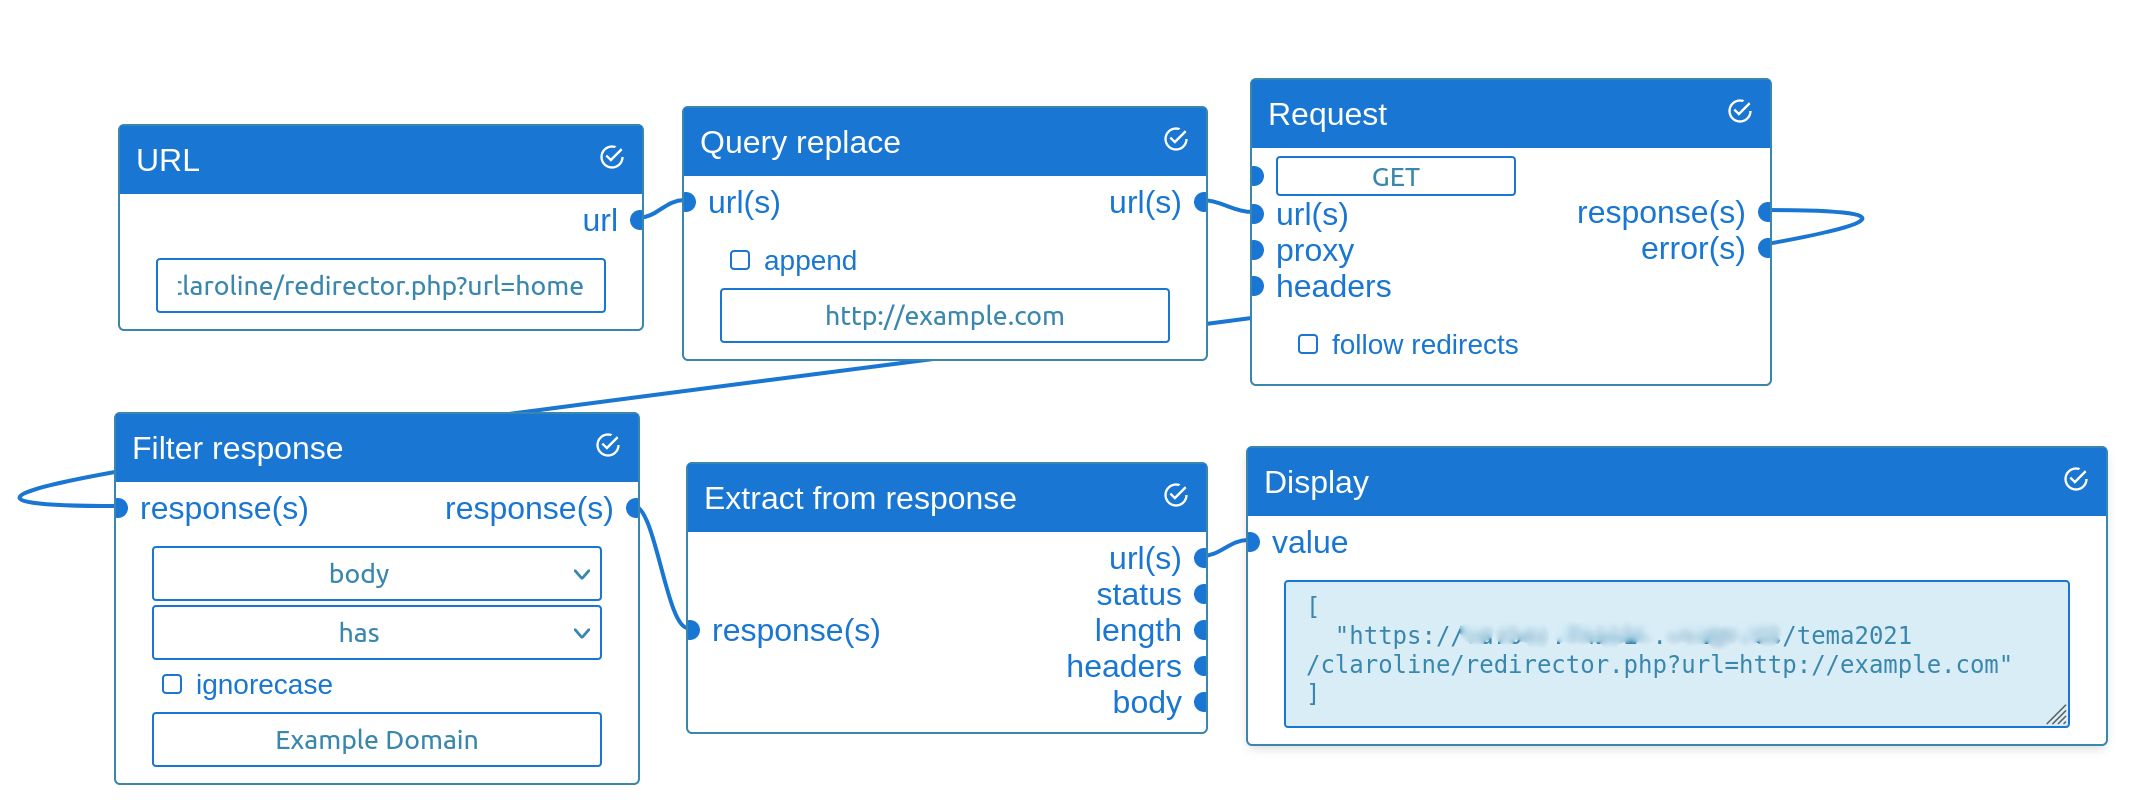
\includegraphics[width=15cm]{img/tables/43_Recipe-OpenRedirect.png}
    \caption{Receta: Vulnerabilidad \textit{OpenRedirect}.}
    \label{fig:openredirect}
\end{figure}

\subsection{Llamadas a la \textit{API}} \label{sub:apicalls}

Al tratarse de un servicio web, es posible realizar llamadas a la \textit{API} sin necesidad de hacer uso de la interfaz. Esta opción está enfocada en los usuario más avanzados que requieran automatizar su flujo de trabajo mediante \textit{scripts}.\sn

Para ello, es necesario realizar una petición \textit{HTTP} usando el método \textit{POST}. Además, la petición debe incluir la cabecera ``\textit{X-Powered-By: Masterchef!}'' y enviar la consulta en formato \textit{JSON}.\sn

Las peticiones actualmente soportadas son\footnote{Los \textit{endpoints} se encuentran detallados en profundidad en el archivo \textit{swagger.yml}}:

\begin{table}[H]
    \begin{center}
        \begin{tabularx}{\textwidth}{| l | l | X |}
            \hline
            \multicolumn{3}{c}{ \textbf{/api/v1/request} } \\
            \multicolumn{3}{c}{Realiza peticiones \textit{HTTP}} \\ \hline
            \textbf{Parámetro} & \textbf{Tipo} & \textbf{Descripción} \\ \hline
            urls & array[url] & Listado de \textit{URLs} objetivo \\ \hline
            method & string & Verbo \textit{HTTP} \\ \hline
            proxy & url & Proxy por el cual enviar las consultas \\ \hline
            headers & map[string]string & Cabeceras \textit{HTTP}. \\ \hline
        \end{tabularx}
    \end{center}
    \caption{\textit{Endpoint} /request}
    \label{tab:endpointrequest}
\end{table}

\begin{table}[H]
    \begin{center}
        \begin{tabularx}{\textwidth}{| l | l | X |}
            \hline
            \multicolumn{3}{c}{ \textbf{/api/v1/lookup/dns} } \\
            \multicolumn{3}{c}{Realiza consultas inversas de \textit{DNS}} \\ \hline
            \textbf{Parámetro} & \textbf{Tipo} & \textbf{Descripción} \\ \hline
            ips & array[ip] & Listado de \textit{IPs} \\ \hline
        \end{tabularx}
    \end{center}
    \caption{\textit{Endpoint} /lookup/dns}
    \label{tab:endpointdns}
\end{table}

\begin{table}[H]
    \begin{center}
        \begin{tabularx}{\textwidth}{| l | l | X |}
            \hline
            \multicolumn{3}{c}{ \textbf{/api/v1/lookup/ips} } \\
            \multicolumn{3}{c}{Realiza consultas de \textit{IP}} \\ \hline
            \textbf{Parámetro} & \textbf{Tipo} & \textbf{Descripción} \\ \hline
            domains & array[domain] & Listado de dominios \\ \hline
        \end{tabularx}
    \end{center}
    \caption{\textit{Endpoint} /lookup/ips}
    \label{tab:endpointips}
\end{table}

\begin{table}[H]
    \begin{center}
        \begin{tabularx}{\textwidth}{| l | l | X |}
            \hline
            \multicolumn{3}{c}{ \textbf{/api/v1/stealth/spider} } \\
            \multicolumn{3}{c}{Obtiene un listado de activos usando fuentes abiertas} \\ \hline
            \textbf{Parámetro} & \textbf{Tipo} & \textbf{Descripción} \\ \hline
            domains & array[domain] & Listado de dominios \\ \hline
            provider & string & Proveedor de búsqueda \\ \hline
            includeSubdomains & boolean & Incluir subdominios \\ \hline
        \end{tabularx}
    \end{center}
    \caption{\textit{Endpoint} /stealth/spider}
    \label{tab:endpointspider}
\end{table}

\begin{table}[H]
    \begin{center}
        \begin{tabularx}{\textwidth}{| l | l | X |}
            \hline
            \multicolumn{3}{c}{ \textbf{/api/v1/stealth/subdomainer} } \\
            \multicolumn{3}{c}{Obtiene un listado de subdominios usando fuentes abiertas} \\ \hline
            \textbf{Parámetro} & \textbf{Tipo} & \textbf{Descripción} \\ \hline
            domains & array[domain] & Listado de dominios \\ \hline
            provider & string & Proveedor de búsqueda \\ \hline
        \end{tabularx}
    \end{center}
    \caption{\textit{Endpoint} /stealth/subdomainer}
    \label{tab:endpointsubdomainer}
\end{table}

Los servicios disponibles a través de la \textit{API} devuelven el código de estado \textbf{404} si no se ha realizado una petición correcta (error en la ruta, método o cabeceras); \textbf{406}, si no se incluyen los parámetros necesarios; o \textbf{200}, si la consulta se ha realizado correctamente.\sn

La figura \ref{fig:apicall} muestra un ejemplo de petición a través de comandos.\sn

\begin{figure}[H]
    \centering
    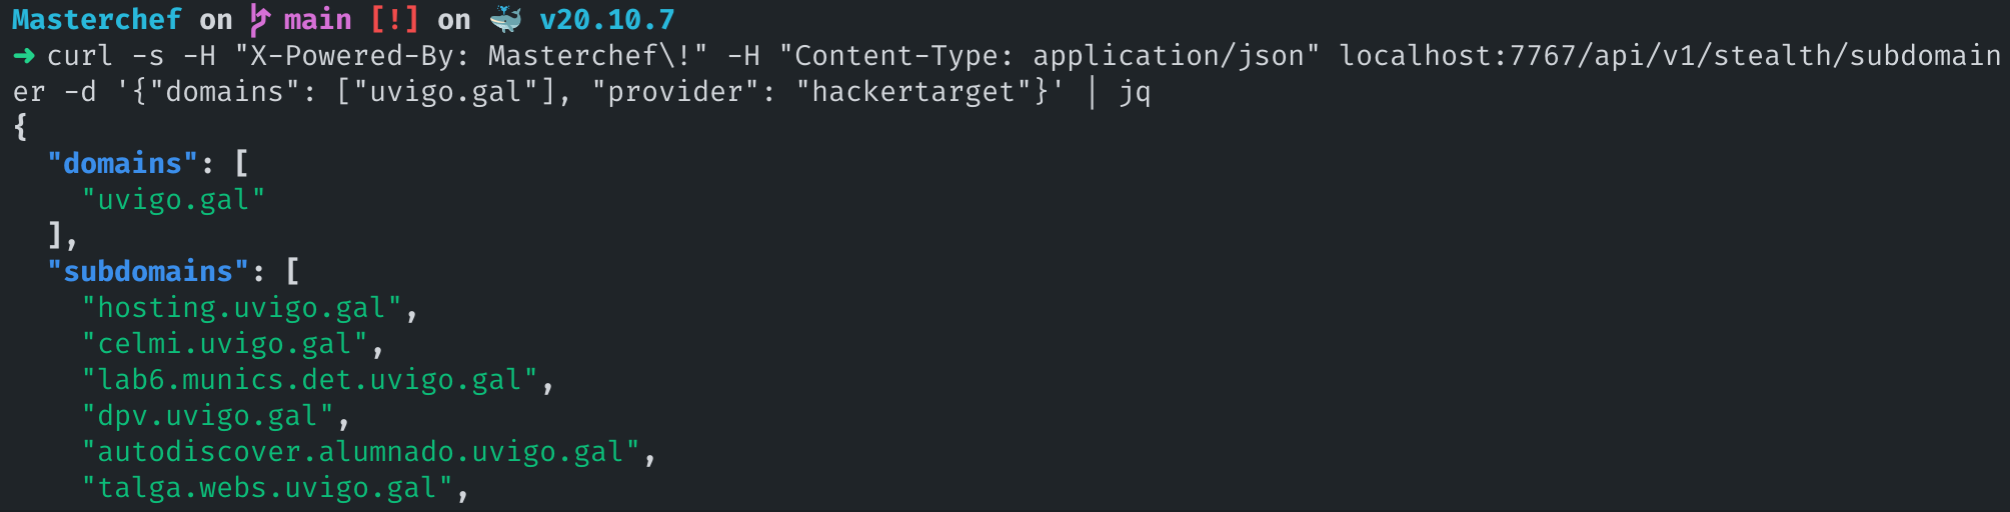
\includegraphics[width=15cm]{img/tables/44_API-Subdomainer.png}
    \caption{Llamada al \textit{subdomainer} a través de \textit{curl}.}
    \label{fig:apicall}
\end{figure}

\newpage

\subsection{Especificación de nuevos \textit{ingredientes}} \label{sub:ingredientspec}

Los tipos de ingredientes están especificados en el archivo \textit{/frontend/src/assets/ingredients.yml}. Actualmente no es posible modificar los ingredientes en soluciones precompiladas. Las especificaciones siguen un formato \textit{YAML}.\sn

Para crear un nuevo tipo de ingrediente, es necesario definir los siguientes valores. Los campos opcionales se marcan con una interrogación (?):\sn

\begin{itemize}
\item \textbf{id}? \ldots Identificador único (sin uso, por el momento).
\item \textbf{name} \ldots Nombre del ingrediente.
\item \textbf{category} \ldots Categoria a la que pertenece.
\item \textbf{aliases} \ldots Etiquetas de búsqueda.
\item \textbf{description} \ldots Descripción de la funcionalidad del ingrediente.
\item \textbf{outputs}? \ldots Conexiones de salida.
    \begin{itemize}
    \item \textbf{name} \ldots Nombre de la conexión.
    \item \textbf{type} \ldots Tipo de la conexión.
    \end{itemize}
\item \textbf{inputs}? \ldots Conexiones de entrada.
    \begin{itemize}
    \item \textbf{name} \ldots Nombre de la conexión.
    \item \textbf{type} \ldots Tipo de la conexión.
    \item \textbf{control}? \ldots Formulario para la modificación de valores por defecto.
        \begin{itemize}
        \item \textbf{type} \ldots Tipo de control.
        \item \textbf{options}? \ldots Valores de configuración del control.
        \end{itemize}
    \end{itemize}
\item \textbf{controls}? \ldots Formularios con los valores de configuración.
    \begin{itemize}
    \item \textbf{name} \ldots Nombre del control.
    \item \textbf{type} \ldots Tipo de control.
    \item \textbf{options}? \ldots Valores de configuración del control.
    \end{itemize}
\item \textbf{code} \ldots Código \textit{JavaScript} para procesar los datos.
\end{itemize}

El campo \textbf{code} cuenta con una serie de variables globales que permiten el acceso a los datos del nodo: \textbf{inputs} (datos de entrada), \textbf{outputs} (datos de salida), \textbf{node.data} (valor de los controles) y \textbf{call} (llamadas a la \textit{API}).\sn

Un ejemplo de especificación de un ingrediente es el mostrado en la figura \ref{fig:ingredientspec}.\n
    \blankpage
    \fancyhead[RE]{\thechapter\hspace{20pt}|\hspace{20pt}OWASP -- WEB SECURITY TESTING GUIDE}
    %%%%%%%%%%%%%%%%%%%%%%%%%%%%%%%%%%%%%%%%%%%%%%%%%%%%%%%%%%%%%%%%%%
%%  ~ Trabajo de Fin de Grado - Universidad de Vigo (ESEI) ~    %%
%% Autor: Diego Enrique Fontán Lorenzo                          %%
%% Tutor: Miguel Ramón Díaz-Cacho Medina                        %%
%% Convocatoria: Julio 2020/21                                  %%
%% Título: Framework de automatización de auditorías Red Team   %%
%%%%%%%%%%%%%%%%%%%%%%%%%%%%%%%%%%%%%%%%%%%%%%%%%%%%%%%%%%%%%%%%%%

%%%%%%%%%%%%%%%%%%%%%%%%%%%%%
%% OWASP
%%%%%%%%%%%%%%%%%%%%%%%%%%%%%

\chapter{OWASP -- Web Security Testing Guide} \label{anx:owasp}

En este anexo, se resumen algunas de las categorías habituales durante un \textit{pentesting} según la metodología \textit{OWASP}. En concreto, se hace referencia a la \textit{Web Security Testing Guide v4.2}. El documento original completo se puede encontrar en la siguiente dirección web: \url{https://owasp.org/www-project-web-security-testing-guide/v42/}.

\section{Contextualización} \label{sec:owaspdef}

\begin{quotation}
    \textit{``El Proyecto de Pruebas OWASP ha estado en desarrollo durante muchos años. El objetivo del proyecto es ayudar a la gente a entender el qué, el por qué, el cuándo, el dónde y el cómo de las pruebas de las aplicaciones web. El proyecto ha proporcionado un marco de pruebas completo, no sólo una simple lista de comprobación o una prescripción de cuestiones que deben abordarse. Los lectores pueden utilizar este marco como plantilla para construir sus propios programas de pruebas o para calificar los procesos de otras personas. La Guía de Pruebas describe con detalle tanto el marco general de pruebas como las técnicas necesarias para ponerlo en práctica.''} -- \textit{OWASP}
\end{quotation}

Hay que entender que las pruebas de seguridad nunca serán una ciencia exacta. No es posible llegar a definir una lista concreta con todos los posibles problemas que deben intentar solucionarse.\sn

El objetivo de la \textit{OWASP WSTG} es intentar recopilar el mayor número de pruebas, explicar las técnicas necesarias y mantener la guía actualizada. El método de pruebas de seguridad de aplicaciones web de \textbf{\textit{OWASP} se basa en el enfoque de caja negra}, es decir, el auditor no sabe nada o tiene muy poca información sobre la aplicación que va a probar.

\section{Categorías} \label{sec:owaspcat}

Las pruebas contenidas en la guía se agrupan por escenarios. Cada escenario tiene un identificador único, en el formato \textbf{WSTG-\textit{categoría}-\textit{control}}. La categoría es  una cadena de 4 caracteres en mayúsculas que identifica el tipo de prueba o debilidad, y el control es un número del 01 al 99. Por ejemplo: \textit{WSTG-INFO-03} es la tercera prueba de la categoría \textit{Recopilación de Información}.\n

La versión 4.2, usada como referencia durante el proyecto, consta de un total de noventa y siete controles, algunos de ellos con múltiples pruebas. Estos controles están agrupados dentro de doce categorías diferentes.\sn

La aplicación presentada como resultado del Trabajo de Fin de Grado descrito en este documento ofrece algunos \textit{ingredientes} ya definidos con los que poder realizar parte de los controles.\sn

Las pruebas cubiertas mediante estos nodos son los siguientes \tab{owaspingredients}.\sn

\begin{table}[H]
    \centering
    \begin{tabularx}{\textwidth}{| l | X |}
        \hline
        \multicolumn{2}{c}{ \textbf{Ingredientes de la categoría \textit{OWASP}} } \\ \hline
        \textbf{Identificador} & \textbf{Descripción} \\ \hline
        WSTG-INFO-01 & Reconocimiento con motores de búsqueda \\ \hline
        WSTG-INFO-02 (1) & \textit{Fingerprint} del servidor web \\ \hline
        WSTG-INFO-03 & Revisión de los archivos de \textit{metainformación} \\ \hline
        WSTG-INFO-04 (1) & Enumeración de aplicaciones web en diferentes \textit{URLs} \\ \hline
        WSTG-INFO-04 (2) & Enumeración de aplicaciones web en diferentes \textit{puertos} \\ \hline
        WSTG-INFO-04 (3) & Enumeración de aplicaciones web usando \textit{hosts} virtuales \\ \hline
        WSTG-INFO-05 & Revisión del contenido de la página web \\ \hline
    \end{tabularx}
    \caption{Ingredientes de la categoría \textit{OWASP}}
    \label{tab:owaspingredients}
\end{table}

Un ejemplo del uso de estos nodos mediante la aplicación es el mostrado en la figura \fig{owaspexample}.\sn

\begin{figure}[H]
    \centering
    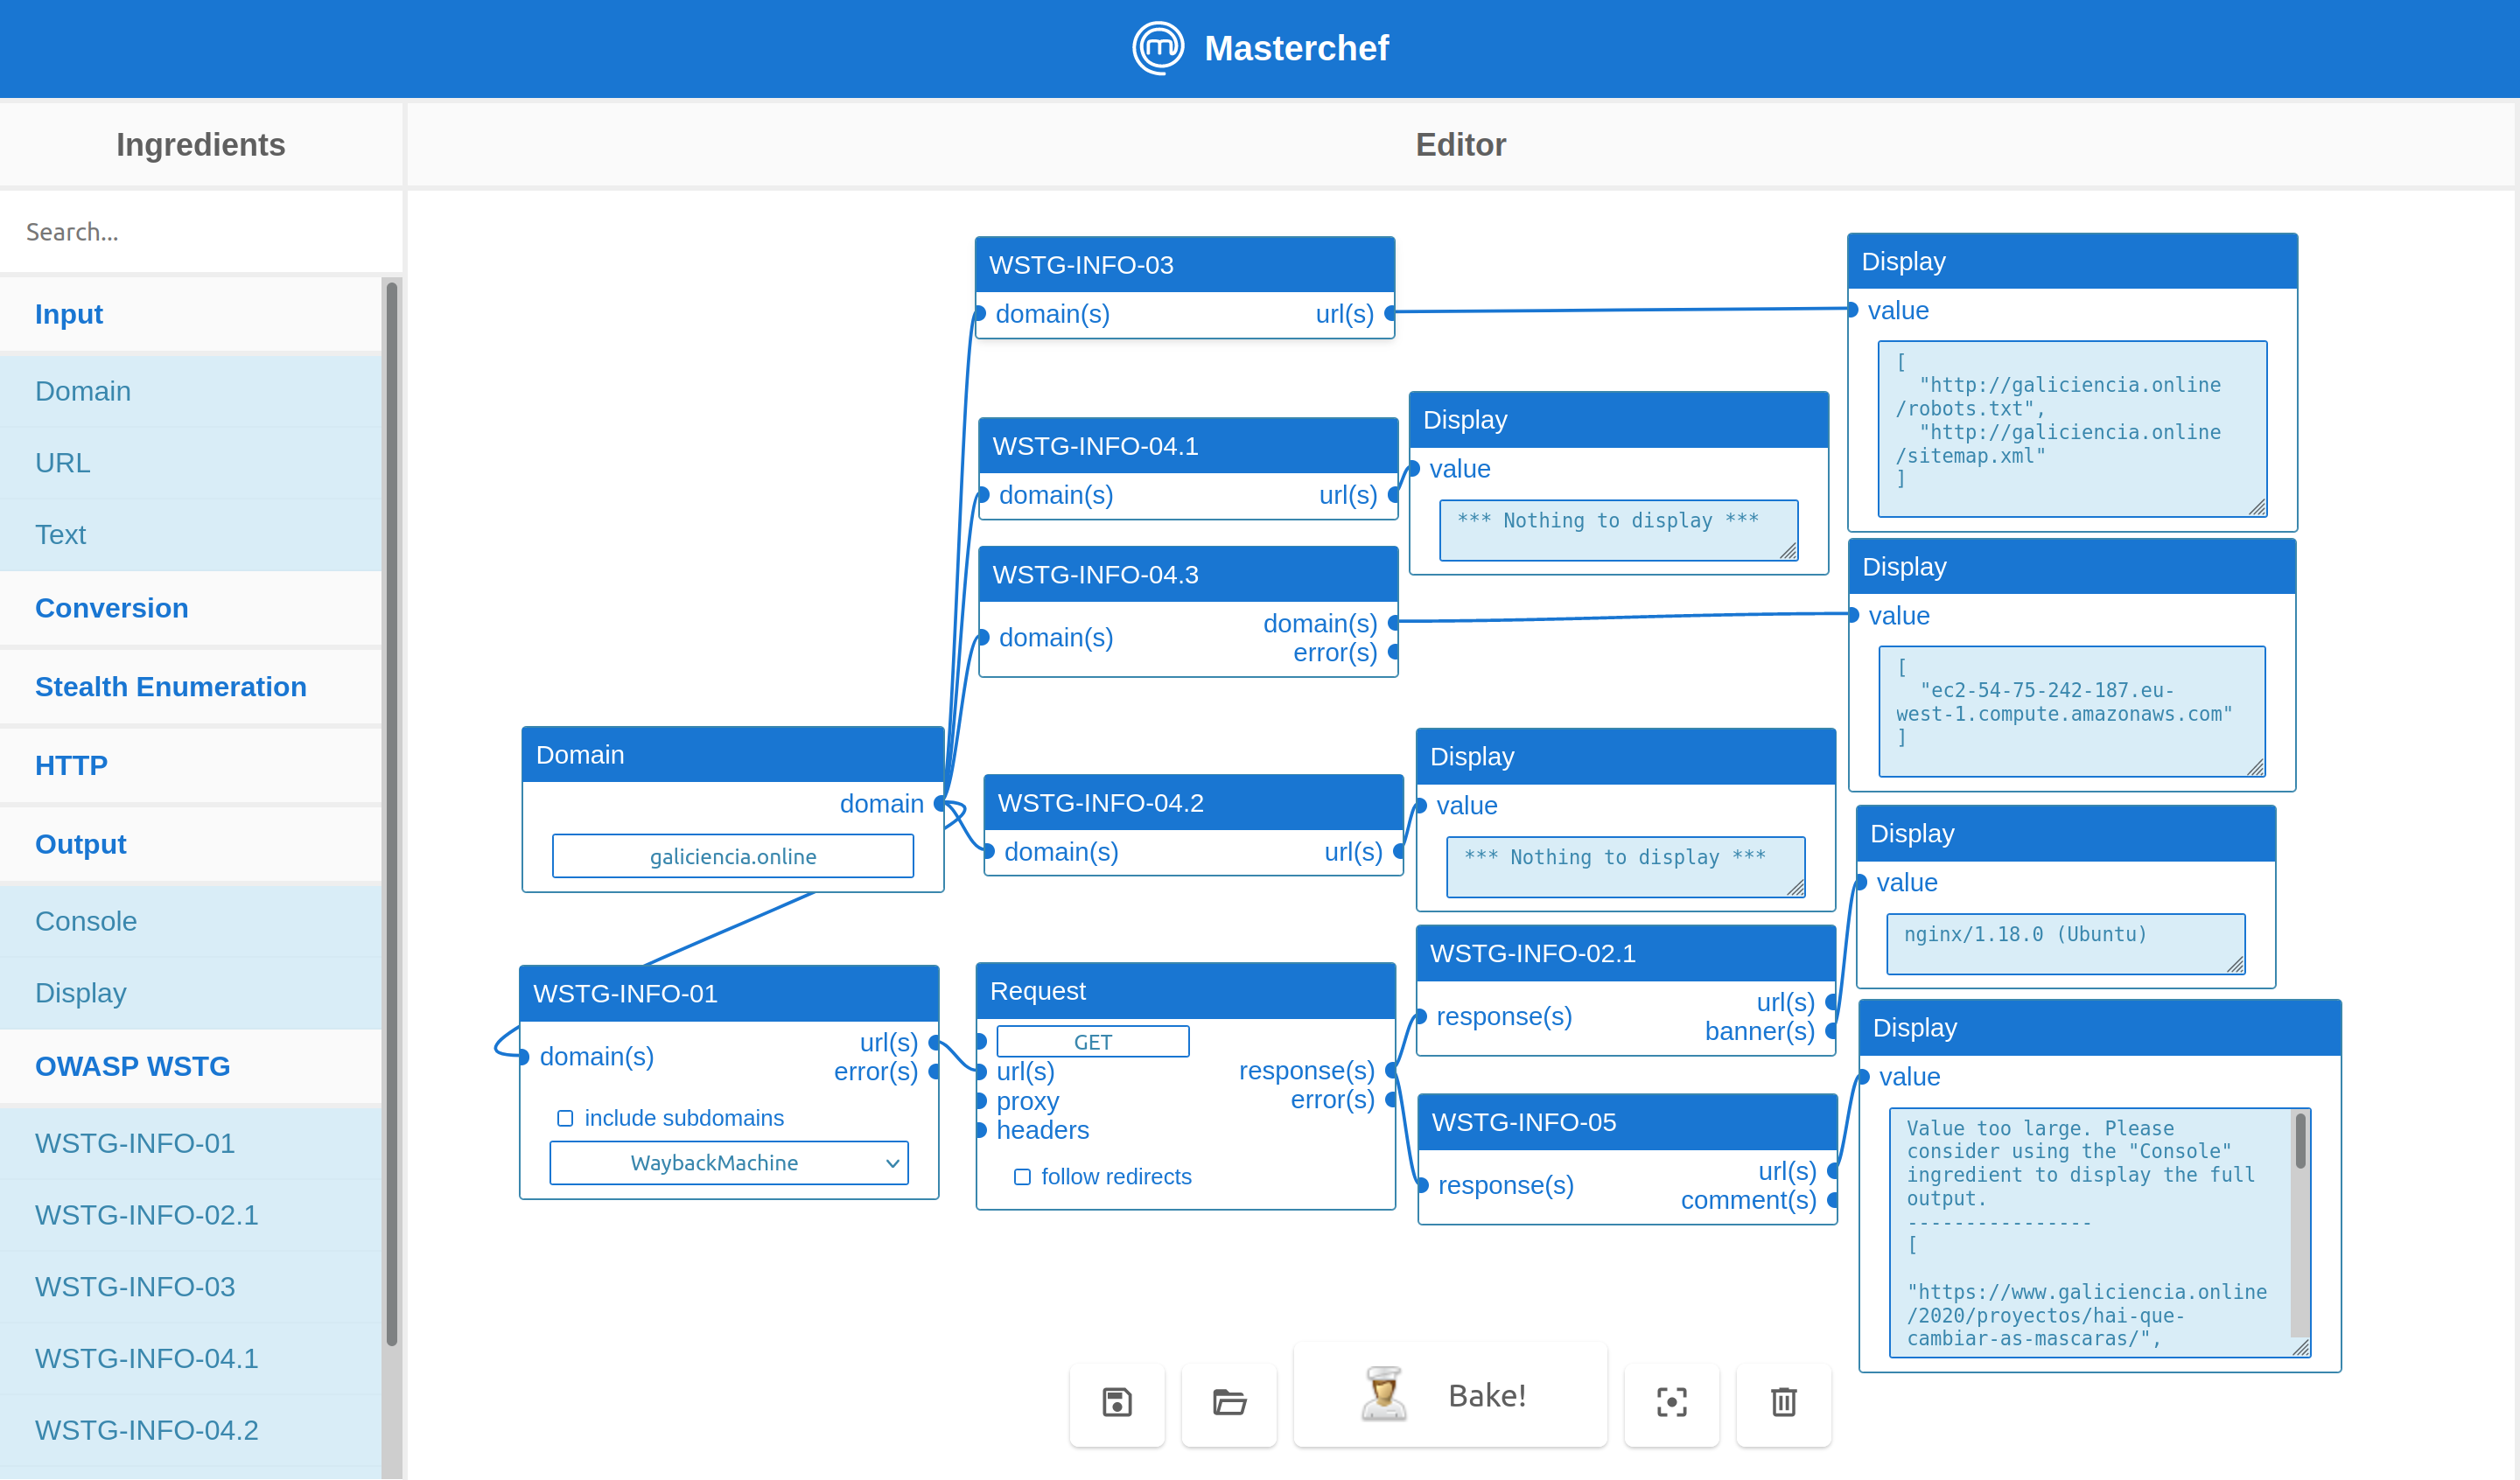
\includegraphics[width=15cm]{img/tables/34_Recipe-WSTG.png}
    \caption{Controles \textit{INFO} de \textit{OWASP WSGT}.}
    \label{fig:owaspexample}
\end{figure}
\end{document}